	\documentclass[11pt]{article}

\usepackage{amssymb,amsmath,amsthm}
\usepackage{verbatim}
\usepackage{fullpage}
\usepackage{gencor}
\usepackage{mathrsfs}
\usepackage{authblk}
\usepackage{graphicx}
\usepackage{caption}
\usepackage{subcaption}
\usepackage{multirow}
\usepackage[nottoc,notlof,notlot,numbib]{tocbibind}
\usepackage{xr-hyper}
\externaldocument[supp-]{supp}
\makeatletter
\renewcommand*{\@fnsymbol}[1]{\ensuremath{\ifcase#1\or *\or**\or\dagger\or \ddagger\or
   \mathsection\or \mathparagraph\or \|\or **\or \dagger\dagger
   \or \ddagger\ddagger \else\@ctrerr\fi}}
 \newcommand{\beginsupplement}{%
        \setcounter{table}{0}
        \renewcommand{\thetable}{S\arabic{table}}%
        \setcounter{figure}{0}
        \renewcommand{\thefigure}{S\arabic{figure}}%
     }

\makeatother

\frenchspacing
\title{An Atlas of Genetic Correlations across Human Diseases and Traits}
\author[1,2,3]{Brendan Bulik-Sullivan$^{\dagger}$\thanks{Co-first authors}$^,$}
\author[*,4]{Hilary K Finucane}
\author[1,2,3]{Verneri Anttila}
\author[5,6]{Alexander Gusev}
\author[7]{Felix R. Day}
\author[8]{ReproGen Consortium}
\author[8]{Psychiatric Genomics Consortium}
\author[8]{Genetic Consortium for Anorexia Nervosa of the Wellcome Trust Case Control Consortium 3}
\author[7]{John R.B. Perry}
\author[1]{Nick Patterson}
\author[1,2,3]{Elise Robinson}
\author[1,2,3]{Mark J Daly}
\author[1,5,6]{Alkes L Price\thanks{Co-last authors}$^,$}
\author[**,1,2,3]{Benjamin M Neale\thanks{Address correspondence to BBS (\texttt{bulik@broadinstitute.org}) or BMN (\texttt{bneale@broadinstitute.org}).}}

\affil[1]{\small{Program in Medical and Population Genetics, Broad Institute of MIT and Harvard, Cambridge, MA, USA}}
\affil[2]{Stanley Center for Psychiatric Genetics, Broad Institute of MIT and Harvard, Cambridge, MA, USA}
\affil[3]{Analytic and Translational Genetics Unit, Massachusetts General Hospital and Harvard Medical School, Boston, Massachusetts, USA.}
\affil[4]{Department of Mathematics, Massachusetts Institute of Technology, Cambridge, MA, USA.}
\affil[5]{Department of Epidemiology, Harvard T.H. Chan School of Public Health, Boston, MA, USA.}
\affil[6]{Department of Biostatistics, Harvard T.H. Chan School of Public Health, Boston, MA, USA.}
\affil[7]{MRC Epidemiology Unit, University of Cambridge School of Clinical Medicine, Institute of Metabolic Science, Cambridge Biomedical Campus, Cambridge, CB2 0QQ, UK}
\affil[8]{A list of members and affiliations appears in the Supplementary Note.}
\date{}
\begin{document}
\maketitle

\begin{abstract}
A recent focus in statistical genetics has been combining genetic association results from multiple phenotypes in order understand the relationships among traits.
In this paper, 
we estimate 300 genetic correlations among 25 traits, totaling more than 1.5 million unique phenotype measurements.
To enable this analysis, we introduce a statistical method based on LD Score regression for estimating genetic correlation using only GWAS summary statistics.
Our results include a positive genetic correlation between anorexia nervosa and schizophrenia and a negative genetic correlation between anorexia nervosa and body mass index, as well as a large number of replications and positive controls. 
These results highlight the power of a polygenic modeling framework, since there currently are no genome-wide significant SNPs for anorexia nervosa. 
 
\end{abstract}
\newpage
%%%%%%%%%%%%%%%%%%%%%%%%%%%%%%%%%%%%%%%%%%%%%%%%%%%%%%%%%%%%%%%
\section*{Introduction}
\label{Introduction}
%%%%%%%%%%%%%%%%%%%%%%%%%%%%%%%%%%%%%%%%%%%%%%%%%%%%%%%%%%%%%%%

Discovering correlations between phenotypes is a fundamental goal of epidemiology, 
with applications to classification and treatment of disease, as well as to development of pharmaceutical drugs.  
One classical strategy in epidemiology is to search for correlations between phenotypes via cross-sectional or longitudinal observational studies; 
however, the interpretation of results from these studies can be confounded and are vulnerable to reverse causation  \cite{smith2003mendelian, smith2014mendelian}. 
An alternative strategy that is effective for heritable traits and is more robust to confounding is to search instead for pairs of phenotypes with shared genetic etiology. 

The earliest methods for searching for traits with genetic overlap were twin and family studies \cite{vandenberg1965multivariate, 
kempthorne1961interpretation,
loehlin1966genetic,
neale1992methodology,
lichtenstein2009common},
which have been applied to a wide spectrum of traits.
However, family methods have the disadvantage of requiring measurements of different traits on the same individuals.
Genome-wide association studies (GWAS) produce effect-size estimates for specific genetic variants, so it is possible to test for shared genetic
etiology using these effect-size estimates, circumventing the requirement to measure multiple traits per individual.
This can substantially reduce the cost and difficulty of epidemiological studies for uncommon diseases and traits that are expensive to assay.

One widely-used technique for testing relationships between phenotypes using GWAS data is Mendelian randomization  
\cite{smith2003mendelian, smith2014mendelian}, which is the specialization to genetics of instrumental variables \cite{angrist2008mostly}.
Mendelian randomization has proved effective for traits for which large-effect genetic variants have been identified \cite{voight2012plasma,do2013common};
however for many complex traits, the heritability is distributed over thousands of variants with small effects \cite{visscher2012five},
in which case Mendelian randomization using genome-wide significant SNPs suffers from low power and weak instrument bias \cite{angrist2008mostly}.

In this paper, our goal is to estimate genetic correlation, a quantity whose definition includes the effects of all SNPs, including those that do not reach genome-wide significance (Methods).
In cases where two phenotypes are suspected of having a cause-effect relationship,
genetic correlation can be interpreted as a re-scaling of the instrumental variables estimate obtained from an instrument constructed using all SNPs (Methods);
however, unlike instrumental variables, genetic correlation is also meaningful for pairs of diseases, and can be interpreted as a genetic analogue of comorbidity.
The two main existing techniques for estimating genetic correlation from GWAS data are restricted maximum likelihood (REML) \cite{yang2010, yang2011gcta, lee2012estimation, pgccdg2013, vattikuti2012heritability, chen2014estimation}
and polygenic scores \cite{purcell2009common, dudbridge2013power}.
These methods have only been applied to a small number of traits so far, 
because they require individual genotypes, 
which are often difficult to obtain due to privacy considerations and informed consent limitations. 

Here, we introduce a computationally fast method based on LD Score regression \cite{buliksullivan2014} for estimating genetic correlation.
This method requires only GWAS summary statistics and is not biased by sample overlap.
We apply this method to data from 25 GWAS and report genetic correlations between 300 pairs of phenotypes. 

%%%%%%%%%%%%%%%%%%%%%%%%%%%%%%%%%%%%%%%%%%%%%%%%%%%%%%%%%%%%%%%
\section*{Results}\label{Results}
%%%%%%%%%%%%%%%%%%%%%%%%%%%%%%%%%%%%%%%%%%%%%%%%%%%%%%%%%%%%%%%

\subsection*{Overview of Methods}

Our method for estimating genetic correlation from summary statistics relies on the fact that the GWAS effect-size estimate for a given SNP incorporates the effects of all SNPs in LD with that SNP \cite{yang2011genomic,buliksullivan2014}. 
For a polygenic trait, SNPs in regions with strong LD will have higher $\chi^2$-statistics on average than SNPs in regions with little LD \cite{buliksullivan2014}. 
A similar relationship holds if we replace $\chi^2$-statistics for a single study with the product of $z$-scores from two different studies.

More precisely, under a polygenic model \cite{yang2010,lee2012estimation}, the expected value of $z_{1j}z_{2j}$ is 
\begin{equation}\label{reg_eqn}
	\E[z_{1j}z_{2j}] = \dfrac{\sqrt{N_1N_2}\rho_g}{M}\ell_j + \dfrac{\rho N_s}{\sqrt{N_1N_2}},
\end{equation}
where $N_i$ is the sample size for study $i$, $\rho_g$ is genetic covariance (defined in Methods), $\ell_j$ is LD Score \cite{buliksullivan2014}, $N_s$ is the number of samples shared between study 1 and study 2, and $\rho$ is the phenotypic correlation among the $N_s$ overlapping samples (Supplementary Note).
If study 1 and study 2 are the same study, then this reduces to the single-phenotype result from \cite{buliksullivan2014}, because the genetic covariance between a trait and itself is the same as heritability, and $\chi^2 = z^2$.
As a consequence of equation 1, we can estimate genetic covariance using the slope from the regression of $z_{1j}z_{2j}$ on LD Score, which is computationally very fast (see Methods). 
If we normalize genetic covariance to lie in the interval $[-1,1]$, we obtain genetic correlation: 
$r_g := \rho_g/\sqrt{h^2_1h^2_2},$ where $h^2_i$ denotes the SNP-heritability from study $i$ \cite{yang2010}. 
Theory and extensive simulations confirm that our method produces robust estimates of genetic correlation, even when summary statistics are affected by population stratification \cite{buliksullivan2014} or sample overlap (Supplementary Note).


\subsection*{Simulations}\label{Simulations}
We performed a series of simulations to evaluate the robustness of the model to potential confounders such as sample overlap
and misspecified models of genetic architecture, as well as to determine whether the inference procedure produces appropriate type I error, 

Estimates of heritability and genetic covariance can be biased if the underlying model of genetic architecture is misspecified
\cite{speed2012improved}; however,
estimates of genetic correlation are more robust to model misspecification biases than estimates of 
heritability or genetic covariance. 
Since genetic correlation is estimated as a ratio,
model misspecification biases that affect the numerator and the denominator in the same direction will tend to cancel. 
In situations where MAF- or LD-dependent genetic architectures are a particular concern, it is possible to correct for such biases 
with LD Score regression using a MAF or LD binning approach (see \cite{finucane2014partitioning} and Online Methods)
similar to that taken by Lee, \emph{et al.} with REML \cite{lee2013estimation}. 

To quantify the bias introduced by MAF- or LD-dependent genetic architectures, we simulated a variety of different LD Scores and genetic architectures.
In realistic scenarios, only a subset of causal SNPs are directly genotyped or successfully imputed, 
so we used a densely imputed panel of 1000 Genomes (1kG) SNPs \cite{10002012integrated} in order to generate phenotypes
and estimate LD Scores, 
but computed summary statistics only for the 16\% of 1kG SNPs that are also in HapMap3 (HM3) \cite{international2010integrating} with MAF above 5\%.
Results from these simulations are displayed in Supplementary Tables 
\ref{parallel}, \ref{antiparallel} and \ref{depcor}.

We found that the partitioned LD Scores were not biased by MAF- and LD-dependent genetic architectures
when estimating heritability and genetic covariance, but gave substantially higher standard errors than non-partitioned LD Scores.
The estimates of genetic correlation from the simpler non-partitioned LD Scores were approximately unbiased in simulations 
where both heritability and genetic covariance depended on LD, and only minimally biased in simulations where genetic 
correlation also depended on LD. In addition, the non-partitioned LD Scores gave substantially lower standard errors than the
more complex partitioned LD Score models.
Thus for the remainder of this paper, we use non-partitioned LD Scores for estimating $r_g$, since these LD Scores had minimal
bias and the lowest variance in simulations.

In all of the simulations described in this section, 
there was full sample overlap, which confirms that the LD Score regression with unconstrained intercept is not biased by sample overlap.


\subsection*{Replication of Pyschiatric Cross-Disorder Results}\label{PGCCDG}

For additional validation, we replicated the estimates of genetic correlations between psychiatric disorders obtained with
individual genotypes and REML by the Psychiatric Genomics Consortium (PGC) \cite{pgccdg2013}, 
by applying LD Score regression to summary statistics generated from the same data \cite{cross2013identification}.
Since these summary statistics were generated from non-overlapping samples, 
we applied LD Score regression using both unconstrained and constrained intercepts (Methods).
Results from these analyses are displayed in Figure \ref{Fig:Replication of PGC Cross-Disorder Results}.
As expected, the genetic correlation estimates from LD Score regression were similar to the results from REML.
LD Score regression with constrained intercept gave standard errors that were only slightly larger than REML,
while the standard errors from LD Score regression with intercept were larger, especially for traits with small sample sizes
(\emph{e.g.,} ADD, ASD).


% Figure 1 -- replication of PGC-CDG results
\begin{figure}[!ht]
\begin{centering}
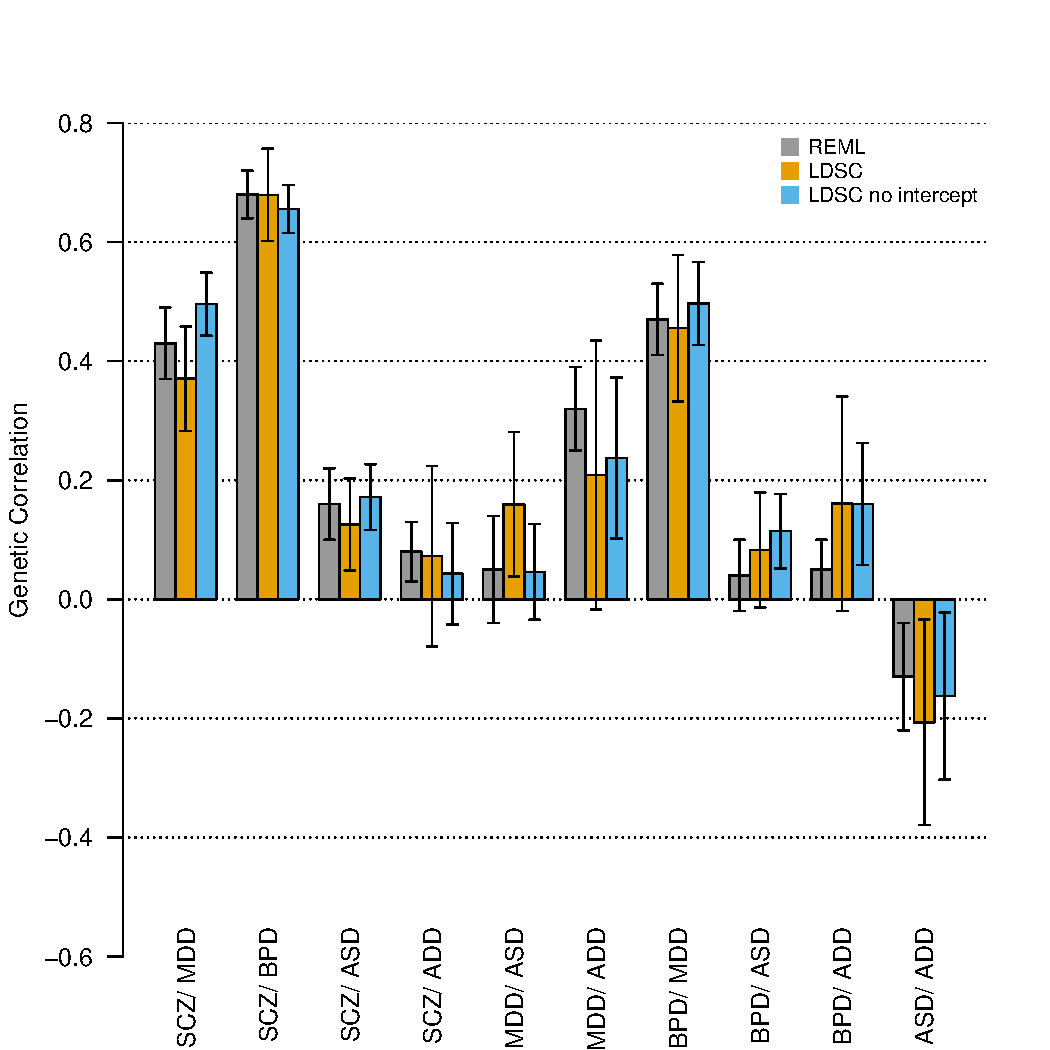
\includegraphics[scale=0.9]{figs/ldsc_vs_gcta.pdf}
\end{centering}
\caption{\label{Fig:Replication of PGC Cross-Disorder Results}\small{\textit{Replication of PGC Cross-Disorder Results.
This plot compares LD Score regression estimates of genetic correlation using the summary statistics from \cite{cross2013identification} (which were generated from approximately the same data as \cite{pgccdg2013}) to 
estimates obtained from REML in \cite{pgccdg2013}.
The horizontal axis indicates pairs of phenotypes, and the vertical axis indicates genetic correlation.
The error bars show standard errors.
Colors indicate different estimation procedures. Green is REML,
orange is LD Score with intercept and white is LD Score with constrained intercept.
The estimates of genetic correlation between psychiatric phenotypes in figure \ref{Fig:300 Gencors} use larger sample sizes;
this plot is intended primarily as a technical validation.
Abbreviations: 
ADD = attention deficit hyperactivity disorder;
ASD = autism spectrum disorder;
BPD = bipolar disorder;
MDD = major depressive disorder;
SCZ = schizophrenia.}}}
\end{figure}

\subsection*{Application to Summary Statistics From 25 Phenotypes}

We used LD Score regression to estimate genetic correlations among 25 phenotypes (URLs, Methods).
Genetic correlation estimates for all 300 pairwise combinations of the 25 traits are displayed in Figure \ref{Fig:300 Gencors}.
For clarity of presentation, 
the 25 phenotypes were restricted to contain only one phenotype from each cluster of highly correlated phenotypes (Methods).
Highly correlated educational, anthropometric, smoking, and insulin-related phenotypes that were excluded from Figure \ref{Fig:300 Gencors}
are displayed in Table \ref{edu} and Figures \ref{giant}, \ref{smoking} and \ref{insulin}, respectively.
References and sample sizes are displayed in Table \ref{N}.

% Figure 2 -- Genetic correlation heatmap with 25 traits
\begin{figure}[!ht]
\begin{centering}
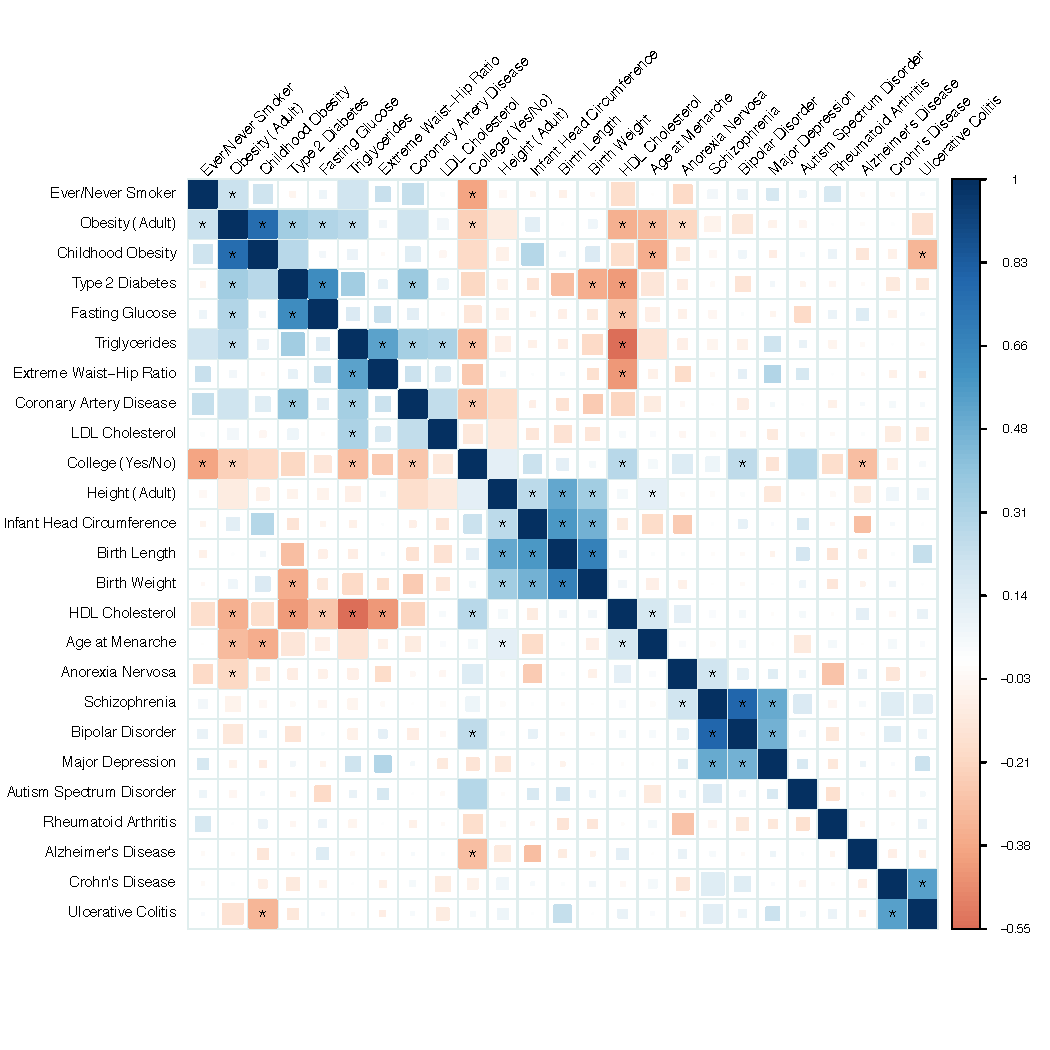
\includegraphics[scale=0.9]{figs/rg_heatmap.pdf}

\caption{         
\label{Fig:300 Gencors}
\small{\textit{Genetic Correlations among 25 Published GWAS.
Blue corresponds to positive genetic correlations; red corresponds to negative genetic correlation. 
Larger squares correspond to more significant $p$-values.
Genetic correlations that are different from zero at 1\% FDR are displayed as full-sized squares. 
Genetic correlations that are significantly different from zero at significance level 0.05 after Bonferroni correction for the 300 tests in this figure are given an asterisk. 
We display results that do not pass multiple testing correction as smaller squares in order to avoid the confusion that would result from whiting our positive controls that do not pass multiple testing correction because of small sample size.
This multiple testing correction is conservative, since the tests are not independent.}}}
\end{centering}
\end{figure}

% Results that are consistent with top SNP results or MR analyses 
For the majority of pairs of traits in Figure \ref{Fig:300 Gencors}, no GWAS-based genetic correlation estimate has been reported; 
however, many associations have been described in an \emph{ad-hoc} manner based off the observation of overlap among genome-wide significant loci.
Examples of genetic correlations that are consistent with overlap among top loci include the correlations between plasma lipids and cardiovascular disease \cite{do2013common}; age at onset of menarche and obesity \cite{perry2014parent}; type 2 diabetes, obesity, fasting glucose, plasma lipids and cardiovascular disease \cite{morris2012large}; birth weight, adult height and type 2 diabetes \cite{horikoshi2013new}; birth length, adult height and infant head circumference \cite{early2012genome, taal2012common}; and childhood obesity and adult obesity \cite{early2012genome}. 
For many of these pairs of traits, we can reject the null hypothesis of zero genetic correlation with overwhelming statistical
significance (\emph{e.g.,} $p<10^{-20}$ for age at onset of menarche and obesity).

% Table 1 -- interesting genetic correlation results highlighted in the main text
\begin{table}[h!]
\centering
\begin{tabular}{ l|llll}
 & Phenotype 1 & Phenotype 2 & $r_g$ (se) & $p$-value \\
\hline
\multirow{13}{*}{Epidemiological} 
& Age at Menarche & Height (Adult) & 0.11 (0.03) & $6\times10^{-5\ **}$  \\
& Age at Menarche & Type 2 Diabetes & -0.13 (0.04) & $3\times10^{-3}$  \\
& Age at Menarche & Triglycerides & -0.15 (0.04) & $1\times10^{-3\ *}$ \\
& Coronary Artery Disease & Age at Menarche &  -0.11 (0.05) & $4\times10^{-2}$ \\
& Coronary Artery Disease & College (Yes/No) & -0.278 (0.07) & $1\times10^{-4\ **}$ \\
& Coronary Artery Disease & Height (Adult) &  -0.17 (0.05) & $2\times10^{-4\ *}$\\
& Alzheimer's & College (Yes/No) & -0.30 (0.08) & $1\times10^{-4\ **}$ \\
& Bipolar Disorder & College (Yes/No) & 0.026 (0.064) & $6\times10^{-5\ **}$ \\
& Obesity (Adult) & College (Yes/No) & -0.23 (0.04) & $2\times10^{-8\ **}$\\
& Triglycerides & College (Yes/No) &-0.30 (0.04)&$5\times10^{-12\ **}$ \\
& Anorexia Nervosa & Obesity (Adult) & -0.20 (0.04) & $4\times10^{-6\ **}$ \\
& Ever/Never Smoker & College (Yes/No) & -0.39 (0.07) & $1\times10^{-9\ **}$ \\
& Ever/Never Smoker & Obesity (Adult) & 0.22 (0.05) & $7\times10^{-5\ **}$ \\
\hline
\multirow{3}{*}{Novel/Nonzero} 
& Autism Spectrum Disorder & College (Yes/No) & 0.28 (0.08) & $5\times10^{-4\ *}$\\
& Ulcerative Colitis & Childhood Obesity & -0.33 (0.08) & $3.9\times10^{-5\ **}$\\
& Anorexia Nervosa & Schizophrenia & 0.19 (0.04)  & $1.5\times10^{-5\ **}$ \\
\hline
\multirow{8}{*}{Novel/Zero} 
& Schizophrenia &Alzheimer's &  0.05 (0.05) & 0.58 \\
& Schizophrenia & Ever/Never Smoker & 0.03 (0.06) & 0.26 \\
& Schizophrenia & Triglycerides & -0.05 (0.04) & 0.21 \\
& Schizophrenia & LDL Cholesterol & -0.02 (0.03) & 0.64 \\
& Schizophrenia & HDL Cholesterol & 0.03 (0.04) & 0.50 \\
& Schizophrenia & Rheumatoid Arthritis & -0.05 (0.05) & 0.38 \\
& Crohn's Disease & Rheumatoid Arthritis & -0.02 (0.09) & 0.83 \\
& Ulcerative Colitis & Rheumatoid Arthritis & -0.09 (0.09) & 0.33 \\
\end{tabular}
\caption{
\small{\textit{\label{table:results}Genetic correlation estimates, standard errors and $p$-values for selected pairs of traits. Results are grouped into
 genetic correlations that are novel genetic results, but are consistent with established epidemiological associations (``Epidemiological''), novel genetic correlations (``Novel/Nonzero'') and interesting null results (``Novel/Zero''). 
 The $p$-values displayed are uncorrected $p$-values.
Results that pass multiple testing correction for the 300 tests in Figure \ref{Fig:300 Gencors} at 1\% FDR are given a single asterisk; results that pass Bonferroni correction at significance level 0.05 are given two asterisks.
For completeness, we present some genetic correlations that are directionally consistent with epidemiological associations but that do not pass multiple testing correction in our data. }}}
\end{table}

% Novel genetic results that are not novel epidemiological results
The first section of table \ref{table:results} lists genetic correlation results that are consistent with well-known epidemiological associations, 
but, as far as we are aware, have not previously been reported using genetic data.
Our estimates of the genetic correlation between age at onset of menarche and adult height \cite{onland2005age}, cardiovascular disease \cite{day2014} and type 2 diabetes \cite{day2014, elks2013age} are consistent with the epidemiological associations. 
Our estimate of a negative genetic correlation between AN and obesity (and a similar genetic correlation with BMI) is intriguing given that the most striking feature of anorexia nervosa is the ability to maintain dangerously low BMI \cite{american2013dsm} and suggests that similar genetic factors may influence normal variation in BMI as well as severely dysregulated BMI in psychiatric illness.
This result is consistent with our observation that BMI GWAS findings appear to primarily implicate neuronal, rather than metabolic, cell-types and epigenetic marks 
\cite{finucane2014partitioning}.
The negative genetic correlation between adult height and coronary artery disease agrees with a replicated epidemiological association  \cite{wang2011associations,hebert1993height,rich1995height}.
We observe several significant associations with the educational attainment phenotypes from
Rietveld \emph{et al.} \cite{rietveld2013gwas}.
We estimate a statistically significant negative genetic correlation between college and Alzheimer's disease, 
consistent with the epidemiological observation that low educational attainment is one of the largest risk factors for Alzheimer's
\cite{barnes2011projected, norton2014potential}. 
The positive genetic correlation between college and bipolar disorder is consistent with psychiatric literature showing that educational attainment and bipolar disorder status are positively correlated
\cite{maccabe2010excellent, tiihonen2005premorbid}, 
Our estimate of a negative genetic correlation between smoking and college is consistent with the epidemiological result that smoking is more prevalent among less-educated groups \cite{pierce1989trends}.
Finally, our estimates of genetic correlations among metabolic traits are consistent with the estimates obtained using REML in Vattikuti \emph{et al.}
\cite{vattikuti2012heritability} (Supplementary Table \ref{vattikuti}), and are directionally consistent with the recent Mendelian randomization results from Wuertz \emph{et al.} \cite{wuertz2014metabolic}.
In addition, our estimate of 0.57 (0.074) for the genetic correlation between Crohn's disease and ulcerative colitis is consistent
with the estimate of 0.62 (0.042) from Chen \emph{et al.} \cite{chen2014estimation}.


% Novel results
The second section of table \ref{table:results} lists results that are, to the best of our knowledge, new both to genetics and epidemiology.
First, we find a positive genetic correlation between anorexia nervosa and schizophrenia.
Comorbidity between eating and psychotic disorders has not been thoroughly investigated in the psychiatric literature \cite{striegel1999psychiatric,blinder2006psychiatric}, and our results raise the intriguing possibility of fundamental similarity between these classes of disease.
Second, we estimate a negative genetic correlation between ulcerative colitis and childhood obesity.
The relationship between premorbid BMI and ulcerative colitis is at present not well-understood,
and our results suggest that exploring this relationship may be a fruitful direction for further investigation. 
Third, we estimate a positive genetic correlation between autism spectrum disorder (ASD) and educational attainment,
which itself has very high genetic correlation with IQ \cite{deary2007intelligence, calvin2010sex, rietveld2013gwas}.
The ASD summary statistics were generated using a case-pseudocontrol study design, so this result cannot be explained by diagnostic biases, such as the tendency for the parents of children who receive a diagnosis of ASD to be better educated than the general population \cite{durkin2010socioeconomic}. 
The distribution of IQ among individuals with ASD has lower mean than the general population, but with heavy tails \cite{robinson2014autism} (\emph{i.e.,} an excess of individuals with extremely low and extremely high IQ).
In addition, there is evidence that the genetic architectures of high IQ and low IQ ASD are dissimilar \cite{samocha2014framework}.
We are unable to offer an explanation for this result, but propose that further exploration of this genetic correlation is an interesting direction for future research.

% Interesting null results
The third section of table \ref{table:results} lists several instances where the genetic correlation is close to zero with small standard error, in contrast to previous reports of epidemiological correlation or pleiotropy.
We estimate genetic correlations close to zero between schizophrenia and rheumatoid arthritis, schizophrenia and smoking, and schizophrenia and plasma lipids. The lack of genetic correlation between schizophrenia and rheumatoid arthritis is interesting because schizophrenia has been observed to be protective for rheumatoid arthritis \cite{silman2002epidemiology}.
The absence of genetic correlation between schizophrenia and smoking is notable because of the high prevalence of smoking among individuals with schizophrenia \cite{de2005meta}. 
Our estimate of zero genetic correlation between schizophrenia and plasma lipid levels or cardiovascular disease contrasts with earlier reports of extensive pleiotropy between schizophrenia and triglycerides \cite{andreassen2013improved2}. 
However, the observation from Andreassen, \emph{et al.} \cite{andreassen2013improved2} could potentially be explained the sensitivity of the method used in the original report to the properties of a few regions with high linkage disequilibrium, 
rather than trait biology (Table \ref{qq_tg}).
We estimate near-zero genetic correlation between Alzheimer's disease and schizophrenia. 
The genetic correlations between Alzheimers disease and the other four psychiatric traits (anorexia nervosa, bipolar, major depression, ASD) are also
close to zero, but with larger standard errors, due to smaller sample sizes.
This suggests that the genetic basis of Alzheimer's disease is distinct from psychiatric conditions. 
Last, we estimate near zero genetic correlation between rheumatoid arthritis and both Crohn's disease and ulcerative colitis. Although these immune diseases share a large number of associated loci \cite{cotsapas2011pervasive,farh2014genetic}, 
it is as often the case that an allele that is risk-increasing for one immune disease is protective for another as an allele is 
risk-increasing for two \cite{cotsapas2011pervasive}, consistent near-zero genetic correlation overall.
This is an example of pleiotropy without genetic correlation (Methods).
%%% Getting # of overlapping gwsig loci w/ concordant and discordant effects from Mark D

 
%%%%%%%%%%%%%%%%%%%%%%%%%%%%%%%%%%%%%%%%%%%%%%%%%%%%%%%%%%%%%%%
\section*{Discussion}\label{Discussion}
%%%%%%%%%%%%%%%%%%%%%%%%%%%%%%%%%%%%%%%%%%%%%%%%%%%%%%%%%%%%%%%\


% Summary of major findings
We have described a new method for estimating genetic correlation from GWAS summary statistics.
We applied our method to a large dataset of publicly available GWAS summary statistics, spanning 25 traits and more than 1.5 million phenotype-genotype pairs. 
We replicated many previously-reported GWAS-based genetic correlations, and confirm observations of overlap among genome-wide significant SNPs, 
Mendelian randomization results and known epidemiological associations, thus validating the utility of genetic correlation as an epidemiological tool.
In addition, we report several novel results that merit further analysis, including a positive genetic correlation between educational attainment and autism spectrum disorder
and a positive genetic correlation between anorexia nervosa and schizophrenia.

% Importance of findings 
This method is an advance for several reasons: 
it does not require individual genotypes, genome-wide significant SNPs or measuring all traits on all individuals;
it is not biased by sample overlap; 
and it is computationally trivial.  
Although it may be possible to extend existing methods such as LD-pruned polygenic scores to work on pairs of summary statistics, 
such methods would be biased by sample overlap, and would suffer from the disadvantage that LD-pruning results in loss of information.
These advantages allow estimation of genetic correlations between a much large set of pairs of phenotypes than was previously possible.

% Limitations of Genetic Correlation
In general, the difficulties in interpreting genetic correlation are similar to the difficulties in interpretation of Mendelian randomization.
Although genetic correlation is immune to environmental confounding, 
genetic correlation is still subject to genetic confounding, 
which is similar to the idea of confounding by pleiotropy from the Mendelian randomization literature (Methods).
This is best illustrated with an example. 
% Alkes suggested moving this example to the supplement in order to obtain a shorter discussion. I think it is a very important
% point, and prefer to leave it in the main text. Ben also seems keen to leave it in.
The negative genetic correlation between HDL and CAD in Figure \ref{Fig:300 Gencors} could result from a direct causal effect $\mathrm{HDL}\rightarrow\mathrm{CAD}$,
but could also result from non-causal shared genetic etiology, 
perhaps mediated by the genetic correlation of -0.55 between HDL and triglycerides (TG),
which is the explanation offered in \cite{do2013common, burgess2014using}. 
This scenario can be represented graphically as 
$\mathrm{HDL}\leftarrow\mathrm{G}\rightarrow\mathrm{TG}\rightarrow\mathrm{CAD}$, 
where $\mathrm{G}$ is the set of genetic variants with effects on both HDL and TG.
This diagram would result in a genetic correlation between HDL and CAD, because there is an unblocked path from HDL to CAD \cite{greenland1999causal}.
Extending genetic correlation to deal with multiple phenotypes that share causal loci 
(\emph{e.g.,} genetic correlation between HDL and CAD controlling for TG, 
analogous to \cite{do2013common,burgess2014using}) is an important direction for future work.

% Limitations of the Method
We note several limitations of the LD Score regression estimator of genetic correlation.
First, LD Score regression requires larger sample sizes than methods such as REML that use individual genotypes
in order to give estimates with acceptable standard error.
Second, LD Score regression is only currently applicable to studies that sample individuals from non-admixed populations
for which a sequenced reference panel (such as 1000 Genomes \cite{10002012integrated}) is available \cite{buliksullivan2014}.
Third, LD Score regression performs optimally when applied to traits with highly polygenic genetic architectures, such as 
psychiatric traits. 
At very large sample size and for less-polygenic traits,
analyzing only the significantly associated SNPs can sometimes be a more powerful strategy.
Developing methods that can make optimal use of both confidently associated large-effect SNPs and diffuse polygenic signal from thousands of small-effect SNPs is a direction for future research.
Fifth, although LD Score regression is not biased by oversampling of cases in case-control studies,
the results may nonetheless be biased by more subtle biases in ascertainment, such as misclassification of cases \cite{pgccdg2013}.

Despite these limitations, we believe that the LD Score regression estimator of genetic correlation will be a useful addition
to the epidemiological toolbox, since it allows for rapid screening for correlations among a diverse set of traits, without the 
need for measuring multiple traits on the same individuals or genome-wide significant SNPs.

%%% INSERT CONCLUSION HERE

\newpage
%%%%%%%%%%%%%%%%%%%%%%%%%%%%%%%%%%%%%%%%%%%%%%%%%%%%%%%%%%%%%%%
\section*{Methods}\label{Methods}
%%%%%%%%%%%%%%%%%%%%%%%%%%%%%%%%%%%%%%%%%%%%%%%%%%%%%%%%%%%%%%%

\subsection*{Definition of Genetic Covariance and Correlation}

Let $S$ denote a set of $M$ SNPs, 
let $X$ denote a vector of additively (0-1-2) coded genotypes for the SNPs in $S$, 
and let $y_1$ and $y_2$ denote phenotypes. Define $\beta := \mathrm{argmax}_{\alpha\in\R^M} \corr\left[y_1, X\alpha\right]^2$,
where the maximization is performed in the population (\emph{i.e.,} in the infinite data limit). 
Let $\gamma$ denote the corresponding vector for $y_2$.
This is a projection, so $\beta$ is unique modulo SNPs in perfect LD. 
Define $h^2_S$, the heritability explained by SNPs in $S$, as $h^2_S(y_1) := \sum_j \beta_j^2$, and the genetic covariance among SNPs in $S$ is defined
$\rho_S(y_1,y_2) := \sum_{j\in S} \beta_j\gamma_j$.
The genetic correlation among SNPs in $S$ is $r_S(y_1,y_2) := \rho_S(y_1,y_2)/\sqrt{h^2_S(y_1)h^2_S(y_2)}$, 
which lies in [-1,1]. 
Following \cite{yang2010}, we use subscript $g$ (as in $h^2_g,\rho_g,r_g$) when the set of SNPs is 
genotyped and imputed SNPs in GWAS.

SNP genetic correlation ($r_g$) is different from family study genetic correlation.
In a family study, the relationship matrix captures information about all genetic variation, 
not just common SNPs. 
As a result, family studies estimate the total [narrow-sense] genetic correlation ($S$ equals all variants).
Unlike the relationship between SNP-heritability \cite{yang2010} and total heritability, 
for which $h^2_g \leq h^2$, 
no similar relationship holds between SNP genetic correlation and total genetic correlation.
If $\beta$ and $\gamma$ are more strongly correlated among common variants than rare variants, then the total genetic correlation will be less than the SNP genetic correlation.

Genetic correlation is (asymptotically) proportional to Mendelian randomization estimates.
If we use a genetic instrument $g_i := \sum_{j\in S} X_{ij}\beta_j$ to estimate the effect $b_{12}$ of $y_1$ on $y_2$,
the 2SLS estimate is $\hat{b}_{2SLS}:=\T{g}y_2/\T{g}y_1$ \cite{angrist2008mostly}.
The expectations of the numerator and denominator are 
$\E[\T{g}y_2]=\rho_S(y_1,y_2)$ and $\E[\T{g}y_1]=h^2_S(y_1)$.
Thus, $\lim_{N\to\infty} \hat{b}_{2SLS} = r_S(y_2,y_1)\sqrt{h^2_S(y_1) / h^2_S(y_2)}$.
If we use the same set $S$ of SNPs to estimate $b_{12}$ and $b_{21}$ (\emph{e.g.,} if $S$ is the set of all common SNPs, as in the genetic correlation analyses in this paper), then this procedure is symmetric in $y_1$ and $y_2$. 

Genetic correlation is different from pleiotropy. 
Two traits have a pleiotropic relationship if many variants affect both.
Genetic correlation is a stronger condition than pleiotropy:
to exhibit genetic correlation, the directions of effect must also be consistently aligned.

%%%%%%%%%%%%%%%%%%%%%%%%%%%%%%%%%%%%%%%%%%%%%%%%%%%%%%%%%%%%%%%
\subsection*{Cross-Trait LD Score Regression} 
%%%%%%%%%%%%%%%%%%%%%%%%%%%%%%%%%%%%%%%%%%%%%%%%%%%%%%%%%%%%%%%

We estimate genetic covariance by regressing $z_{1j}z_{2j}$ against $\ell_j\sqrt{N_{1j}N_{2j}}$,
(where $N_{ij}$ is the sample size for SNP $j$ in study $i$) 
then multiplying the resulting slope by $M$, the number of SNPs in the reference panel with MAF between 5\% and 50\% 
(technically, this is an estimate of $\pf$, see the Supplementary Note).

If we know ahead of time that there is no sample overlap, we can constrain the intercept of this regression to zero, which gives lower standard error. This can be accomplished with the \texttt{--no-intercept}
flag in \texttt{ldsc}.

%%%%%%%%%%%%%%%%%%%%%%%%%%%%%%%%%%%%%%%%%%%%%%%%%%%%%%%%%%%%%%%
\subsection*{Regression Weights} 
%%%%%%%%%%%%%%%%%%%%%%%%%%%%%%%%%%%%%%%%%%%%%%%%%%%%%%%%%%%%%%%

For heritability estimation, we use the regression weights from \cite{buliksullivan2014}. 
If effect sizes for both phenotypes are drawn from a bivariate normal distribution, then
the optimal regression weights for genetic covariance estimation are 
\begin{equation}
\var[z_{1j}z_{2j} \,|\, \ell_j ] \propto
	\left( 
		\frac{N_1\hsqo\ell_j}{M} + 1
	\right) 
	\left(  
		\frac{N_2\hsqt\ell_j}{M} + 1
	\right) 
	+ 					
	2\left( 
		\dfrac{\sqrt{N_1N_2}\rho_g}{M}\ell_j + \dfrac{\rho N_s}{\sqrt{N_1N_2}}
	\right)^2
\end{equation}
(Supplementary Note). This quantity depends on several parameters ($h^2_1,h^2_2,\rho_g,\rho,N_s$)
which are not known a priori, so it is necessary to estimate them from the data.
We compute the weights in two steps:
\begin{enumerate}
\item The first regression is weighted using heritabilities from the single-trait LD Score regressions,
$\rho N_s=0$, and $\rho_g$ estimated as $\hat{\rho}_g := (\lbar\sqrt{N_1N_2})^{-1}\sum_j z_{1j}z_{2j}$.
\item The second regression is weighted using the estimates of $\rho N_s$ and $\rho_g$ from step 1. 
The genetic covariance estimate that we report is the estimate from the second regression.
\end{enumerate}
Linear regression with weights estimated from the data is called feasible generalized least squares (FGLS). 
FGLS has the same limiting distribution as WLS with optimal weights, so WLS $p$-values are valid for FGLS \cite{angrist2008mostly}. 
In addition, we weight by $1/\ell_j$ (where $\ell_j$ is LD Score with sum over regression SNPs) in order to downweight SNPs that are overcounted. 
This is a heuristic: the optimal approach is to rotate the data so that it is de-correlated, 
but this rotation matrix is difficult to compute.

%%%%%%%%%%%%%%%%%%%%%%%%%%%%%%%%%%%%%%%%%%%%%%%%%%%%%%%%%%%%%%%
\subsection*{Assessment of Statistical Significance via Block Jackknife}
%%%%%%%%%%%%%%%%%%%%%%%%%%%%%%%%%%%%%%%%%%%%%%%%%%%%%%%%%%%%%%%

Summary statistics for SNPs in LD are correlated, so the OLS standard error will be biased downwards. 
We estimate a heteroskedasticity-and-correlation-robust standard error with a block jackknife over blocks of adjacent SNPs.
This is the same procedure used in \cite{buliksullivan2014}, and gives accurate standard errors in simulations (Table \ref{se_sim}).
We obtain a standard error for the genetic correlation by using a ratio block jackknife over SNPs.
The default setting in \texttt{ldsc} is 200 blocks per genome, which can be adjusted with the \texttt{--num-blocks} flag.


%%%%%%%%%%%%%%%%%%%%%%%%%%%%%%%%%%%%%%%%%%%%%%%%%%%%%%%%%%%%%%%
\subsection*{Computational Complexity}
%%%%%%%%%%%%%%%%%%%%%%%%%%%%%%%%%%%%%%%%%%%%%%%%%%%%%%%%%%%%%%%

Let $N$ denote sample size and $M$ the number of SNPs. 
The computational complexity of the steps involved in LD Score regression are as follows:
\begin{enumerate}
\itemsep-0.1em
\item Computing summary statistics takes $\mathscr{O}(MN)$ time.
\item Computing LD Scores takes $\mathscr{O}(MN)$ time, though the $N$ for computing LD Scores need not be large. 
We use the $N=378$ Europeans from 1000 Genomes.
\item LD Score regression takes $\mathscr{O}(M)$ time and space.
\end{enumerate}
For a user who has already computed summary statistics and downloads LD Scores from our website (URLs), 
the computational cost of LD Score regression is $\mathscr{O}(M)$ time and space.
For comparison, REML takes time $\mathscr{O}(MN^2)$ for computing the GRM
and $\mathscr{O}(N^3)$ time for maximizing the likelihood.

Practically, estimating LD Scores takes roughly an hour parallelized over chromosomes, and
LD Score regression takes about 15 seconds per pair of phenotypes on a 2014 MacBook Air with 1.7 GhZ Intel Core i7 processor.

%%%%%%%%%%%%%%%%%%%%%%%%%%%%%%%%%%%%%%%%%%%%%%%%%%%%%%%%%%%%%%%
\subsection*{Summary Statistic Datasets}\label{datasets}
%%%%%%%%%%%%%%%%%%%%%%%%%%%%%%%%%%%%%%%%%%%%%%%%%%%%%%%%%%%%%%%

We selected traits for inclusion in the main text via the following procedure:

\begin{enumerate}
\itemsep-0.1em
\item Begin with all publicly available non-sex-stratified European-only summary statistics.
\item Remove studies that do not provide signed summary statistics.
\item Remove studies not imputed to at least HapMap 2.
\item Remove studies that include heritable covariates.
\item Remove all traits with heritability $z$-score below 4. Genetic correlation estimates for traits with heritability $z$-score below 4 are generally too noisy to interpret.
\item Prune clusters of correlated phenotypes (\emph{e.g.,} obesity classes 1-3) by picking the trait from each cluster with the highest heritability heritability $z$-score.
\end{enumerate}

We then applied the following filters (implemented in the script \texttt{sumstats\_to\_chisq.py} included with \texttt{ldsc}):
\begin{enumerate}
\itemsep-0.1em
\item For studies that provide a measure of imputation quality, filter to INFO above 0.9.
\item For studies that provide sample MAF, filter to sample MAF above 1\%.
\item In order to restrict to well-imputed SNPs in studies that do not provide a measure of imputation quality, filter to HapMap3 \cite{international2010integrating} SNPs with 1000 Genomes EUR MAF above 5\%, which tend to be well-imputed in most studies. This 
step should be skipped if INFO scores are available for all studies.
\item If sample size varies from SNP to SNP, remove SNPs with effective sample size less than $0.67$ times the 90th percentile of sample size.
\item Remove indels and structural variants.
\item Remove strand-ambiguous SNPs.
\item Remove SNPs whose alleles do not match the alleles in 1000 Genomes.
\item Because the presence of outliers can increase the regression standard error, we also removed
 SNPs with extremely large effect sizes ($\chi^2 > 80$, as in \cite{buliksullivan2014}).
\end{enumerate}

GC correction at any stage biases the heritability and genetic covariance estimates downwards (see the Supplementary Note of \cite{buliksullivan2014}.
The biases in the numerator and denominator of genetic correlation cancel exactly, 
so genetic correlation is not biased by GC correction. 
A majority of the studies analyzed in this paper used GC correction, 
so we do not report genetic covariance and heritability.

Data on Alzheimer's disease were obtained from the following source:

\begin{quotation}
    \textit{\small{International Genomics of Alzheimer's Project (IGAP) is a large two-stage study based upon genome-wide association studies (GWAS) on individuals of European ancestry. 
    In stage 1, IGAP used genotyped and imputed data on 7,055,881 single nucleotide polymorphisms (SNPs) to meta-analyze four previously-published GWAS datasets consisting of 17,008 Alzheimer's disease cases and 37,154 controls 
    (The European Alzheimer's Disease Initiative, EADI; the Alzheimer Disease Genetics Consortium, ADGC; The Cohorts for Heart and Aging Research in Genomic Epidemiology consortium, CHARGE; The Genetic and Environmental Risk in AD consortium, GERAD). 
    In stage 2, 11,632 SNPs were genotyped and tested for association in an independent set of 8,572 Alzheimer's disease cases and 11,312 controls. 
    Finally, a meta-analysis was performed combining results from stages 1 and 2.}}
\end{quotation}
We only used stage 1 data for LD Score regression.

\newpage

%%%%%%%%%%%%%%%%%%%%%%%%%%%%%%%%%%%%%%%%%%%%%%%%%%%%%%%%%%%%%%%
\section*{URLs}\label{URLs}
%%%%%%%%%%%%%%%%%%%%%%%%%%%%%%%%%%%%%%%%%%%%%%%%%%%%%%%%%%%%%%%
\begin{enumerate}
\itemsep-0.1em

	\item \texttt{ldsc} software:\\ 
		\texttt{github.com/bulik/ldsc}
		
	\item This paper:\\
		\texttt{github.com/bulik/gencor\_tex}
		
	\item PGC (psychiatric) summary statistics:\\ 
		\texttt{www.med.unc.edu/pgc/downloads}
		
	\item GIANT (anthopometric) summary statistics: \\
		\texttt{www.broadinstitute.org/collaboration/giant/index.php/GIANT\_consortium\_data\_files}
	\item EGG (Early Growth Genetics) summary statistics:\\
		\texttt{www.egg-consortium.org/}
	
	\item MAGIC (insulin, glucose) summary statistics: \\
		\texttt{www.magicinvestigators.org/downloads/}
		
	\item CARDIoGRAM (coronary artery disease) summary statistics:\\	
		\texttt{www.cardiogramplusc4d.org}
	
	\item DIAGRAM (T2D) summary statistics:\\
		\texttt{www.diagram-consortium.org}
		
	\item Rheumatoid arthritis summary statistics:\\
		\texttt{www.broadinstitute.org/ftp/pub/rheumatoid\_arthritis/Stahl\_etal\_2010NG/}
	
	\item IGAP (Alzheimers) summary statistics:\\
		\texttt{www.pasteur-lille.fr/en/recherche/u744/igap/igap\_download.php}

	\item IIBDGC (inflammatory bowel disease) summary statistics:\\
		\texttt{www.ibdgenetics.org/downloads.html}\\
		We used a newer version of these data with 1000 Genomes imputation.

	\item Plasma lipid summary statistics:\\
		\texttt{www.broadinstitute.org/mpg/pubs/lipids2010/}
	
	\item SSGAC (educational attainment) summary statistics:\\
		\texttt{www.ssgac.org/}
	
	\item Beans:\\
		\texttt{www.barismo.com}\\
		\texttt{www.bluebottlecoffee.com}
\end{enumerate}

\newpage
%%%%%%%%%%%%%%%%%%%%%%%%%%%%%%%%%%%%%%%%%%%%%%%%%%%%%%%%%%%%%%%
\section*{Acknowledgements}\label{Acknowledgements}
%%%%%%%%%%%%%%%%%%%%%%%%%%%%%%%%%%%%%%%%%%%%%%%%%%%%%%%%%%%%%%%

We would like to thank P. Sullivan, C. Bulik and S. Caldwell for helpful discussion. This work was supported by NIH grants R01 MH101244  (ALP), R03 CA173785 (HKF) and by the Fannie and John Hertz Foundation (HKF). The coffee that Brendan drank while writing this paper was roasted by Barismo in Arlington, MA and Blue Bottle Coffee in Oakland, CA. 

Data on anorexia nervosa were obtained by funding  from the WTCCC3 WT088827/Z/09 titled ``A genome-wide association study of anorexia nervosa''.

Data on glycaemic traits have been contributed by MAGIC investigators and have been downloaded from www.magicinvestigators.org.

Data on coronary artery disease / myocardial infarction have been contributed by CARDIoGRAMplusC4D investigators and have been downloaded from 
\texttt{www.CARDIOGRAMPLUSC4D.ORG}

We thank the International Genomics of Alzheimer's Project (IGAP) for providing summary results data for these analyses. The investigators within IGAP contributed to the design and implementation of IGAP and/or provided data but did not participate in analysis or writing of this report. IGAP was made possible by the generous participation of the control subjects, the patients, and their families. The i-Select chips was funded by the French National Foundation on Alzheimer's disease and related disorders. EADI was supported by the LABEX (laboratory of excellence program investment for the future) DISTALZ grant, Inserm, Institut Pasteur de Lille, Universit� de Lille 2 and the Lille University Hospital. GERAD was supported by the Medical Research Council (Grant 503480), Alzheimer's Research UK (Grant 503176), the Wellcome Trust (Grant 082604/2/07/Z) and German Federal Ministry of Education and Research (BMBF): Competence Network Dementia (CND) grant 01GI0102, 01GI0711, 01GI0420. CHARGE was partly supported by the NIH/NIA grant R01 AG033193 and the NIA AG081220 and AGES contract N01-AG-12100, the NHLBI grant R01 HL105756, the Icelandic Heart Association, and the Erasmus Medical Center and Erasmus University. ADGC was supported by the NIH/NIA grants: U01 AG032984, U24 AG021886, U01 AG016976, and the Alzheimer's Association grant ADGC-10-196728.


%%%%%%%%%%%%%%%%%%%%%%%%%%%%%%%%%%%%%%%%%%%%%%%%%%%%%%%%%%%%%%%
\section*{Author Contributions}\label{author_contribs}
%%%%%%%%%%%%%%%%%%%%%%%%%%%%%%%%%%%%%%%%%%%%%%%%%%%%%%%%%%%%%%%


MJD provided reagents.
BMN and ALP provided reagents.
CL, ER, VA, JP and FD aided in the interpretation of results.
JP and FD provided data on age at onset of menarche.
The caffeine molecule is responsible for all that is good about this manuscript.
BBS and HKF are responsible for the rest.
All authors revised and approved the final manuscript.


%%%%%%%%%%%%%%%%%%%%%%%%%%%%%%%%%%%%%%%%%%%%%%%%%%%%%%%%%%%%%%%
\section*{Competing Financial Interests}
%%%%%%%%%%%%%%%%%%%%%%%%%%%%%%%%%%%%%%%%%%%%%%%%%%%%%%%%%%%%%%%

Unfortunately, we have no financial conflicts of interest to declare.

\newpage
\bibliographystyle{unsrt}
\bibliography{gencor}
\beginsupplement

\newpage
%%%%%%%%%%%%%%%%%%%%%%%%%%%%%%%%%%%%%%%%%%%%%%%%%%%%%%%%%%%%%%%
\section*{Supplementary Note}
%%%%%%%%%%%%%%%%%%%%%%%%%%%%%%%%%%%%%%%%%%%%%%%%%%%%%%%%%%%%%%%

\subsection*{Quantitative Traits}
Suppose we sample two cohorts for two phenotypes,
$y_1$ and $y_2$,
with sample sizes $N_1$ and $N_2$.
We model phenotypes as $y_1 = Y\beta + \delta$,
and $y_2 = Z\gamma + \epsilon$,
where $Y$ and $Z$ are matrices of genotypes normalized to mean zero and variance one\footnote{
We ignore the distinction between normalizing and centering in the population and in the sample, 
since this introduces only $\mathscr{O}(1/N)$ error.},
with dimensions $N_1\times M$ and $N_2\times M$, respectively; 
$\beta$ and $\gamma$ are vectors of per-normalized genotype effect sizes,
and $\delta$ and $\epsilon$ are vectors of environmental or non-additive genetic effects,
In this model, $Y$ and $Z$ are unobserved matrices of all SNPs, including SNPs that are not genotyped.

We treat all of $Y, Z, \beta, \gamma, \delta $ and $\epsilon$ as random.
Suppose that $(\beta, \gamma)$ has mean zero and covariance matrix\
\begin{equation*} 
	\var[(\beta, \gamma)] = \frac{1}{M}
		\left( \begin{array}{cc}
		\hsqo I & \gencov I\\
		\gencov I& \hsqt  I
	\end{array} \right),
\end{equation*}
and $(\delta, \epsilon)$ has mean zero and covariance matrix
\begin{equation*}
	\var[(\delta, \epsilon)] = 
		\left( \begin{array}{cc}
		(1-\hsqo) I & \envcov I\\
		\envcov I& (1-\hsqt) I
	\end{array} \right).
\end{equation*}
Let $\rho := \gencov + \envcov$.
Genotypes are \emph{i.i.d.} draw from a distribution with covariance matrix $R$
(\emph{i.e.,} $r$ is an LD matrix with $r_{jk} = \E[Y_{ij}Y_{ik}]$).
There are $N_s$ individuals included in both studies.

The assumption that all $\beta$ is drawn with equal variance for all SNPs hides an implicit assumption that 
rare SNPs have larger per-allele effect sizes than common SNPs. 
As discussed in the simulations section of the main text and in our earlier work \cite{buliksullivan2014}, LD Score regression is robust to moderate violations of this assumption, though it may break down in extreme
cases, \emph{e.g.,} if all causal variants are rare.
In situations where a different model for $\var[\beta]$ is more appropriate, all proofs in this note go through
with LD Score replaced by weighted LD Scores, $\ell_j = \sum_k \var[\beta_j]r^2_{jk}$.

\begin{lemma} Under this model, the expected genetic covariance between phenotypes is $\gencov$, justifying our use of the notation $\gencov$.
\end{lemma}
\begin{proof} Let $X$ denote an $1\times M$ vector of normalized, centered genotypes for an arbitrary individual. 
Under the model, the additive genetic component of $y_1$ for this individual is $\sum_jX_{j}\beta_j$,
and the additive genetic component of $y_2$ for this individual is $\sum_jX_{j}\gamma_j$.
Thus, the genetic covariance between $y_1$ and $y_2$ is 
\begin{align*}
	\cov\left[\sum_j X_j\beta_j,\sum_j X_j\gamma_j\right] &= 
		\E\left[\left(\sum_j X_j\beta_j\right)\left(\sum_j X_j\gamma_j\right)\right]\\
		&= \sum_j \sum_k \E[X_jX_k\beta_j\gamma_k]\\
		&= \sum_j \E[X_j^2\beta_j\gamma_j]\\
		&= \sum_j \E[X_j^2]\E[\beta_j\gamma_j]\\
		&= \rho_g.
\end{align*}
\end{proof}

We compute linear regression $z$-scores $z_{1j}:= \T{Y}_jy_1/\sqrt{N_1}$ and $z_{2j}:= \T{Y}_jy_2/\sqrt{N_2}$ for genotyped SNPs $j$.
\begin{prop}\label{supp_condexp_qt}
Let $j$ denote a genotyped SNP. Under the model described above, 
\begin{equation}
	\E[z_{1j}z_{2j}] = \frac{\sqrt{N_1N_2}\gencov}{M}\ell_j  + \frac{N_s\rho}{\sqrt{N_1N_2}}.
\end{equation}
\end{prop}

\begin{proof} By the law of total expectation, 
\begin{equation}\label{totalexp}
\E[z_{1j}z_{2j}] = \E[ \E[z_{1j}z_{2j} \,|\, Y, Z ] ]
\end{equation}
\noindent
First we compute the inner expectation from equation \ref{totalexp}, with $Z$ and $Y$ fixed.
\begin{align}
	\E[z_{1j}z_{2j}\,|\,Y,Z] &= \frac{1}{\sqrt{N_1N_2}}\E[\T{Y}_jy_1\T{y_2}Z_j]  \nonumber \\
       		&= \frac{1}{\sqrt{N_1N_2}}\T{Y}_j\E[{(Y\beta+\delta)}\T{(Z\gamma+\epsilon)}]Z_j\nonumber\\
        		&= \frac{1}{\sqrt{N_1N_2}}\T{Y}_j\left(Y\E[\T{\beta}\gamma]Z + \E[\T{\delta} Z\gamma]+\E[\T{\beta}\T{Y}\epsilon]+ \E[\T{\delta}\epsilon]\right)Z_j\nonumber\\
        		&= \frac{1}{\sqrt{N_1N_2}}\T{Y}_j\left(Y\E[\T{\beta}\gamma]Z + \E[\T{\delta}\epsilon]\right)Z_j\nonumber\\
        		&= \frac{1}{\sqrt{N_1N_2}}\left( \frac{\gencov}{M} \T{Y}_jY\T{Z}_jZ  + \envcov\T{Y}_jZ_j  \right).\label{inner}
\end{align}
\noindent
Next, we remove the conditioning on $Y$ and $Z$.
\begin{equation}\label{inner_first}
\frac{1}{\sqrt{N_1N_2}}\E[\T{Y}_jZ_j ] = \frac{N_s}{\sqrt{N_1N_2}},
\end{equation}
and 
\begin{equation}\label{inner_second}
\frac{1}{\sqrt{N_1N_2}}\E[\T{Y}_jY\T{Z}_jZ] = \ell_j + \frac{MN_s}{\sqrt{N_1N_2}}.
\end{equation}
Substituting equations \ref{inner_first} and \ref{inner_second} into equation \ref{inner},
\begin{align}
	\E[z_{1j}z_{2j}] 
&= 
	\frac{\sqrt{N_1N_2}\gencov}{M}\ell_j  + \frac{N_s\left(\rho_g + \rho_e\right)}{\sqrt{N_1N_2}}\nonumber\\
&=
	\frac{\sqrt{N_1N_2}\gencov}{M}\ell_j  + \frac{N_s\rho}{\sqrt{N_1N_2}}.\label{qt_ldscore}
\end{align}
If study 1 and study 2 are the same study, then $N_1=N_2=N_s$, $\rho_g=h^2_g$ and $\rho=1$, so equation \ref{qt_ldscore}
reduces to the LD Score regression equation for a single trait from \cite{buliksullivan2014}.
\end{proof}

%%%%%%%%%%%%%%%%%%%%%%%%%%%%%%%%%%%%%%%%%%%%%%%%%%%%%%%%%%%%%%%
\subsection*{Regression Weights}
%%%%%%%%%%%%%%%%%%%%%%%%%%%%%%%%%%%%%%%%%%%%%%%%%%%%%%%%%%%%%%%

We can improve the efficiency of LD Score regression weighting by the reciprocal of the conditional variance function (CVF),
$\var[z_{1j}z_{2j} \,|\, \ell_j ]$.
The CVF is not uniquely determined by the assumptions about the first and second moments of $\beta$ and $\gamma$ used to derive proposition \ref{supp_condexp_qt}.
Therefore we derive the CVF for the case where 
 $z_{1j}$ and $z_{2j}$ are jointly distributed as bivariate normal\footnote{
For instance, it is sufficient but not necessary to assume that $\beta$, $\gamma$, $\delta$ and $\epsilon$ are multivariate normal.
More generally, the $z$-scores will be approximately normal if $\beta$ and $\gamma$ are reasonably polygenic.
If the distribution of effect sizes is heavy-tailed, \emph{e.g.,} if there are few casual SNPs, then the CVF may be larger.}.

Fom a standard formula for double second moments of the bivariate normal, the CVF is
\begin{align}
	\var[z_{1j}z_{2j} \,|\, \ell_j ] 
&= 
	\E[z_{1j}^2z_{2j}^2]\nonumber\\
&=  
	\var[z_{1j}]\var[z_{2j}]
	+
	2\E[z_{1j}z_{2j}]^2\nonumber\\
&\propto 
	\left( 
		\frac{N_1\hsqo\ell_j}{M} + 1
	\right) 
	\left(  
		\frac{N_2\hsqt\ell_j}{M} + 1
	\right) 
	+ 					
	2\left( 
		\dfrac{\sqrt{N_1N_2}\rho_g}{M}\ell_j + \dfrac{\rho N_s}{\sqrt{N_1N_2}}
	\right)^2
\end{align}
In cases where the normality assumption does not hold, LD Score regression will remain unbiased, but may be inefficient, because the regression weights will be suboptimal.

\subsection*{Liability Threshold Model}

In the liability threshold (probit) model \cite{pearson1901inheritance}, 
binary traits are determined by an unobserved continuous liability $\psi$.
The observed trait is $y := \ind[\psi > \tau]$, where $\tau$ is the liability threshold.
If $\psi$ is normally distributed, then setting $\tau:=\Phi^{-1}(1-K)$ (where $\Phi$ is the standard normal cdf) yields a population prevalence of $K$.

The liability threshold construction is surprisingly general. 
If $y$ is an arbitrary binary phenotype, then we can define a normally distributed liability for $y$ by setting
$\psi_i$ to be a random draw from a normal distribution truncated at the left by $\tau$ if $y_i=1$ and 
truncated at the right by $\tau$ if $y_i=0$.
We prefer to think of liability scale heritability as a useful way to compare the heritabilities of binary phenotypes with different prevalences, rather than a quantity that is only meaningful if one is willing to make strong assumptions about the data generating process.

For phenotypes generated according to the liability threshold model, 
we can estimate not only the heritability and genetic covariance of the observed phenotype, 
but also the heritability and genetic covariance of the unobserved liability.

In the next lemma, we derive population case and control allele frequencies 
in terms of the heritability of liability when liability is generated by a polygenic model.
Since we are only modeling additive effects and are willing to assume Hardy-Weinberg equilibrium,
we lose no generality and simplify notation considerably by stating the proofs in terms of haploid genotypes.

We state this lemma in terms of marginal per-allele effect sizes, instead of the per-normalized-genotype effect sizes considered in the earlier results on quantitative traits.
Here marginal means that these are the effect sizes obtained by univariate regression of phenotype against genotype in the infinite data limit. 
Haploid normalized genotypes are defined $X_j := (G_j - p_j)/\sqrt{p_j(1-p_j)}$.
If $\beta_j$ is the marginal per-normalized-genotype effect and $\zeta_j$ is the marginal per-allele effect, 
we have $X_j\beta_j = G_j\zeta_j$. 
Thus, setting $G_{ij}=1$ yields $\zeta_j = \beta_j\sqrt{(1-p_j)/p_j}$.

\begin{lemma}
Suppose unobserved liabilities $\psi, \varphi$ for traits $y_1,y_2$ with thresholds $\tau_1,\tau_2$ corresponding to prevalences $K_1,K_2$ are generated according to the usual polygenic model for quantitative traits, i.e.,
$\psi_i=\sum_j X_{ij}\beta_j+\delta$, $\varphi_i=\sum_j X_{ij}\gamma_j+\epsilon$, with
\begin{equation*} 
	\var[(\beta, \gamma)] = \frac{1}{M}
		\left( \begin{array}{cc}
		\hsqo I & \gencov I\\
		\gencov I& \hsqt  I
	\end{array} \right),
\end{equation*}
and
\begin{equation*}
	\var[(\delta, \epsilon)] = 
		\left( \begin{array}{cc}
		(1-\hsqo) I & \envcov I\\
		\envcov I& (1-\hsqt) I
	\end{array} \right).
\end{equation*}
Let $\zeta_j$ and $\xi_j$ denote the marginal per-allele effect sizes of $j$ on $\psi$ and $\varphi$, and let $p_{cas,kj}:=\prob[G_{ij}=1\cond y_{ik}=1]$ for $k=1,2$. Then
\begin{align*}
	\E[p_{cas,1j}-p_{con,1j}] &= 0,\\
	\E[p_{cas,2j}-p_{con,2j}] &= 0, \\
	\var[p_{cas,1j}-p_{con,1j}] &= \dfrac{p_j(1-p_j)\phi(\tau_1)^2h^2_1}{MK_1^2(1-K_1)^2)}\ell_j, \\
	\var[p_{cas,2j}-p_{con,2j}] &= \dfrac{p_j(1-p_j)\phi(\tau_2)^2h^2_2}{MK_2^2(1-K_2)^2}\ell_j,\\
	\cov[p_{cas,1j}-p_{con,1j},p_{cas,2j}-p_{con,2j}] &= \dfrac{p_j(1-p_j)\phi(\tau_1)\phi(\tau_2)\rho_g}{MK_1(1-K_1)K_2(1-K_2)}\ell_j,
\end{align*}
where $\phi$ is the standard normal density.
These results apply to population allele frequencies, not allele frequencies in a finite sample. 
We deal with ascertained finite samples in the next section.
\end{lemma}
\begin{proof}
This proof is accomplished in two steps.
First, we compute allele frequencies conditional on the marginal effects on liability. 
To do this, we reverse the conditional probability using Bayes' theorem, 
which reduces the problem to a series of [Taylor approximations to] Gaussian integrals. 
Second, we remove the conditioning on the marginal effects on liability in order to express the 
allele frequencies in terms of $h^2_1,h^2_2,\rho_g$ and $\ell_j$.
Since liability is just a quantitative trait, we need only apply the LD Score regression equation for quantitative traits.

By Bayes' rule, 
\begin{align}
	\prob[G_{ij}=1\cond y_{i1}=1,\zeta_j]
&=
	\dfrac{\prob[y_{i1}=1\cond G_{ij}=1,\zeta_j]\prob[G_{ij}=1]}{\prob[y_{i1}=1]}\nonumber\\
&=
	\dfrac{p_j}{K_1}\prob[y_{i1}=1\cond G_{ij}=1,\zeta_j]\nonumber\\
&=
	\dfrac{p_j}{K_1}\prob[\psi_i>\tau_1\cond G_{ij}=1,\zeta_j].\label{bayesrule}
\end{align}

The distribution of $\psi$ is
$\psi\cond G_{ij}=1,\zeta_j = N(\zeta_j, 1)$ (where the approximation that the variance equals one holds when the marginal heritability explained by $j$ is small, which is the typical case in GWAS).
Thus $\prob[\psi_i>\tau_1\cond G_{ij}=1]$ is simply a Gaussian integral.
We approximate this probability with a first-order Taylor expansion around $\tau_1$.
\begin{align}
	\prob[\psi_i>\tau_1\cond G_{ij}=1,\zeta_j]
&=
	1-\Phi(\tau_1-\zeta_j)\nonumber\\
&\approx
	K_1 + \phi(\tau_1)\zeta_j\label{taylorexp},
\end{align}
Substituting equation \ref{taylorexp} into equation \ref{bayesrule},
\begin{align}
	\prob[G_{ij}=1\cond y_{i1}=1,\zeta_j]
&=
	\dfrac{p_j}{K}\left(K+\phi(\tau_1)\zeta_j\right)\label{case}.
\end{align}
A similar argument shows that 
\begin{align}
	\prob[G_{ij}=1\cond y_{i1}=0,\zeta_j]
&=
	\dfrac{p_j}{1-K_1}\left(1-K-\phi(\tau_1)\zeta_j\right)\label{control}.
\end{align}
Subtracting equation \ref{case} from equation \ref{control},
\begin{align}\label{condprob}
	\prob[G_{ij}=1\cond y_{i1}=1,\zeta_j]-\prob[G_{ij}=1\cond y_{i1}=0,\zeta_j]
&=
	p_j\dfrac{\phi(\tau_1)\zeta_j}{K_1(1-K_1)}.
\end{align}
Similar results hold for trait 2, replacing $\zeta$ with $\xi$ and subscript 1 with subscript 2.

We have written the probabilities in question in terms of constants and marginal effects on liability.
Since liability is simply a quantitative trait, the means, variances, and covariances of the marginal effects on liability
are described by the LD Score regression equation for quantitative traits.
Precisely, $\E[\xi_j]=\E[\zeta_j] = 0$, $\var[\xi_j]=(1-p_j)\hsqo\ell_j/p_kM$, $\var[\zeta_j]=(1-p_j)\hsqt\ell_j/p_jM$ and $\cov[\zeta_j,\xi_j]=(1-p_j)\rho_g\ell_j/p_jM$.
If we combine these results with equation \ref{condprob}, we find that $\E[p_{cas,1j}-p_{con,1j}]=0$;
\begin{align}
	\var[p_{cas,1j}-p_{con,1j}]
&=
	\var\left[\dfrac{p_j\phi(\tau_1)\zeta_j}{K_1(1-K_1)}\right]\nonumber\\
&=
	\dfrac{p_j(1-p_j)\phi(\tau_1)^2h^2_1}{MK_1^2(1-K_1)^2}\ell_j,
\end{align}
(similarly for trait two) and 
\begin{align}
	\cov[p_{cas,1j}-p_{con,1j},p_{cas,2j}-p_{con,2j}]
&=
	\cov\left[\dfrac{p_j\phi(\tau_1)\zeta_j}{K_1(1-K_1)},\dfrac{p_j\phi(\tau_2)\xi_j}{K_2(1-K_2)}\right]\nonumber\\
&=
	\dfrac{p_j(1-p_j)\phi(\tau_1)\phi(\tau_2)\rho_g}{MK_1(1-K_1)K_2(1-K_2)}\ell_j.\label{cov}
\end{align} 
\end{proof}


\subsection*{Ascertained Studies of Liability Threshold Traits}

In the next proposition, we derive an LD Score regression equation for ascertained case/control studies.

Let $P_i$ denote the sample prevalence of $y_i$ in study $i$ for $i=1,2$.
We compute $z$-scores
$$z_j :=\frac {\sqrt{NP(1-P)}(\hat{p}_{cas} - \hat{p}_{con})} {\sqrt{\hat{p}_j(1-\hat{p}_j)}},$$
where $\hat{p}_j$ denotes allele frequency in the entire sample\footnote{
The expected value of $\hat{p}_j$ is not equal to $p_j$ unless $P=K$ or $j$ has zero marginal effect.},
$\hat{p}_{cas}$ denotes sample case allele frequency
and $\hat{p}_{con}$ denotes sample control allele frequency.

We emphasize one subtlety before stating the main proposition. 
The results in this section allow for study $i$ to select samples based on $y_j$ only if $i=j$.
If study 1 ascertains on $y_2$ -- for example, if all cases in study $1$ have $y_1=y_2=1$ -- then 
$\hat{p}_{cas,1j}$ will not be an unbiased estimate of $p_{cas,1j}$.
Indeed, in this example, $\E[\hat{p}_{cas,1j}]=\prob[G_{ij}=1\cond y_1=y_2=1]$, 
which will not equal $p_{cas,1j}=\prob[G_{ij}=1\cond y_1=1]$ unless $\rho=1$ or $\rho=0$.
This follows from the fact that the conditionals and marginals of a bivariate normal are equal iff $\rho=0$ or $\rho=1$.
We do not derive formulae describing the bias, except to note that the most
common scenario, the ``healthy controls'' model -- cases are sampled independently but all controls are controls for both traits -- is probably nothing to worry about.
This is because for binary traits where cases are rare, 
$\prob[G_{ij}=1\cond y_1=0]\approx\prob[G_{ij}=1\cond y_1=y_2=0]$.
Conditioning on $y_2=0$ hardly changes the probability, because $y_2=0$ most of the time, anyway.

\begin{prop}\label{binary_prop}
Under a polygenic model, 
\begin{align}
	\E[z_{1j}z_{2j}]
&\approx
	\dfrac{\sqrt{N_1N_2}\rho_{g,obs}}{M}\ell_j+
	\sqrt{N_1N_2P_1(1-P_1)P_2(1-P_2)}\left(
	\sum_{a,b\in\{cas,con\}}\dfrac{N_{a,b}(-1)^{1+\mathbf{1}[a=b]}}{N_{a,1}N_{b,2}}\right)
\end{align}
where 
\[
\rho_{g,obs} := \rho_g\left(\dfrac{\phi(\tau_1)\phi(\tau_2)\sqrt{P_1(1-P_1)P_2(1-P_2)}}{K_1(1-K_1)K_2(1-K_2)}\right)
\]
denotes observed scale genetic covariance, $N_{a,b}$ denotes the number of individuals with phenotype $a$ in study 1 and $b$ in study two for $a,b\in\{cas,con\}$ (e.g., $N_{cas,con}$ is the number of individuals who are a case in study 1 but a control in study 2).
\end{prop}
\begin{proof}
The full form of $z_{1j}z_{2j}$ is 
\begin{equation*}
	z_{1j}z_{2j} = \dfrac{
	{\sqrt{cN_1N_2}(\hat{p}_{cas,1j} - \hat{p}_{con,1j})(\hat{p}_{cas,2j} - \hat{p}_{con,2j})}}
	{\sqrt{\hat{p}_{1j}(1-\hat{p}_{1j})\hat{p}_{2j}(1-\hat{p}_{2j})}},
\end{equation*}
where $c:=P_1(1-P_1)P_2(1-P_2)$.
Our strategy for obtaining the expectation is
\begin{align}
	\E[z_{1j}z_{2j}]
&\approx
	\sqrt{cN_1N_2}\dfrac{\E[(\hat{p}_{cas,1j} -\hat{p}_{con,1j})(\hat{p}_{cas,2j} - \hat{p}_{con,2j})]}
	{\E[\sqrt{\hat{p}_{1j}(1-\hat{p}_{1j})\hat{p}_{2j}(1-\hat{p}_{2j})]}}\label{ratio}\\
&\approx
	\sqrt{cN_1N_2}\dfrac{\E[(\hat{p}_{cas,1j} -\hat{p}_{con,1j})(\hat{p}_{cas,2j} - \hat{p}_{con,2j})]}
	{\sqrt{\E[\hat{p}_{1j}(1-\hat{p}_{1j})\hat{p}_{2j}(1-\hat{p}_{2j})]}}\label{sqrts}\\
&=
	\sqrt{cN_1N_2}\dfrac{\E\left[\E[(\hat{p}_{cas,1j} -\hat{p}_{con,1j})(\hat{p}_{cas,2j} - \hat{p}_{con,2j})\cond \zeta_j,\xi_j]\right]}
	{\sqrt{\E\left[\E[\hat{p}_{1j}(1-\hat{p}_{1j})\hat{p}_{2j}(1-\hat{p}_{2j})\cond \zeta_j,\xi_j]\right]}}\label{zz_condexp},
\end{align}
where $\zeta_j$ and $\xi_j$ denote the marginal per-allele effects of $j$.
Approximation \ref{ratio} hides $\mathscr{O}(1/N)$ error from moving from the expectation of a ratio to a ratio of expectations.
Approximation \ref{sqrts} hides $\mathscr{O}(1/N)$ error from moving from the expectation of a square root to a square root of expectations.
Equality \ref{zz_condexp} follows from applying of the law of total expectation to the numerator and denominator.

First, we compute the numerator.
By linearity of expectation, 
\begin{align}
	\E[(\hat{p}_{cas,1j} -\hat{p}_{con,1j})(\hat{p}_{cas,2j} - \hat{p}_{con,2j})]\cond \zeta_j,\xi_j]
&=
	\E[\hat{p}_{cas,1j}\hat{p}_{cas,2j}] 
	- 
	\E[\hat{p}_{cas,1j}\hat{p}_{con,2j}]\nonumber\\
	&-
	\E[\hat{p}_{con,1j}\hat{p}_{cas,2j}]
	+
	\E[\hat{p}_{con,1j}\hat{p}_{con,2j}]\label{fourmoreterms}
\end{align}
After conditioning on the marginal effects $\zeta_j$ and $\xi_j$,
the only source of variance in the sample allele frequencies $\hat{p}_{cas,1},\hat{p}_{con,1},\hat{p}_{cas,2},\hat{p}_{con,2}$ is sampling error. 
Write $\hat{p}_{cas,1j}\hat{p}_{cas,2j} = (p_{cas,1j}+\eta)(p_{cas,2j}+\nu)$, 
where $\eta$ and $\nu$ denote sampling error. 
If study 1 and study 2 share samples, 
$\nu$ and $\eta$ will be correlated:
\begin{align}
	\E[\hat{p}_{cas,1j}\hat{p}_{cas,2j}\cond \zeta_j,\xi_j] 
&= 
	p_{cas,1j}p_{cas,2j} + \E[\eta\nu]\nonumber\\
&\approx
	p_{cas,1j}p_{cas,2j} + \dfrac{N_{cas,cas}\sqrt{p_{cas,1j}(1-p_{cas,1j})p_{cas,2j}(1-p_{cas,2j})}}{N_{cas,1}N_{cas,2}}\label{biv_clt}\\
&\approx
	p_{cas,1j}p_{cas,2j}\left(1+ \dfrac{N_{cas,cas}}{N_{cas,1}N_{cas,2}}\right)\label{ignore},
\end{align}
where approximation \ref{biv_clt} is the (bivariate) central limit theorem, 
and approximation \ref{ignore} comes from ignoring the difference between $\sqrt{p_{cas,1j}(1-p_{cas,1j})p_{cas,2j}(1-p_{cas,2j})}$ and $p_j(1-p_j)$. 
This step is justified in the derivation of the denominator.
Similar relationships hold for the other terms in equation \ref{fourmoreterms}.

We can remove the conditioning on $\zeta_j$ and $\xi_j$ using equation \ref{cov}. 
\begin{align}
	\E[(p_{cas,1j} -p_{con,1j})(p_{cas,2j} - p_{con,2j})]
&=
	\dfrac{p_j(1-p_j)\phi(\tau_1)\phi(\tau_2)\rho_g}{MK_1(1-K_1)K_2(1-K_2)}\ell_j\label{remove_cond}.
\end{align}
If we combine equations \ref{ignore} and \ref{remove_cond}, we obtain
\begin{align}\label{numerator}
\E[(\hat{p}_{cas,1j} -\hat{p}_{con,1j})(\hat{p}_{cas,2j} - \hat{p}_{con,2j})]
\approx
p_j(1-p_j)\left(
\dfrac{\phi(\tau_1)\phi(\tau_2)\rho_g}{c'M}\ell_j
+
\sum_{a,b\in\{cas,con\}}\dfrac{N_{a,b}(-1)^{1+\bf{1}[a=b]}}{N_{a,1}N_{b,2}}\right),
\end{align}
where $c':=K_1(1-K_1)K_2(1-K_2)$.

Next, we derive the expectation of the denominator.
Conditional on $\zeta_j$ and $\xi_j$, $\hat{p}_{1j}(1-\hat{p}_{1j})$ is $P_1p_{cas,1j}+ (1-P_1)p_{con,1j}$ plus $\mathscr{O}(1/N)$ sampling 
variance. If studies 1 and 2 share samples, the $\mathscr{O}(1/N)$ sampling variance in $\hat{p}_{1j}(1-\hat{p}_{1j})$ and 
$\hat{p}_{2j}(1-\hat{p}_{2j})$ will be correlated, but this still only amounts to $\mathscr{O}(N_s/N_1N_s)$ error.
If we remove the conditioning on $\zeta_j$ and $\xi_j$, then $P_1p_{cas,1j}+ (1-P_1)p_{con,1j}$ is equal to $p_j(1-p_j)$ plus $\mathscr{O}(h^2_{1,obs}\ell_j/M)$ error from uncertainty in $\zeta_j$.
The covariance between uncertainty in $\zeta_j$ and uncertainty in $\xi_j$ is driven by $\rho_{g,obs}$, so the expectation of the denominator is $\E\left[\sqrt{\hat{p}_{1j}(1-\hat{p}_{1j})\hat{p}_{2j}(1-\hat{p}_{2j})}\right] = p_j(1-p_j)\left(1
+ \mathscr{O}(N_s/N_1N_2) + \mathscr{O}(\rho_{g,obs}\ell_j/M)\right)$.
We make the approximation\footnote{
For $\ell_j=100$ (roughly the median 1kG LD Score), $M=10^7$ and $\rho_{g,obs}=1$, we get $\rho_{g,obs}\ell_j/M=10^{-5}$.
A worst-case value for $N_s/N_1N_2$ might be $N_s=N_1=N_2=10^3$, in which case $N_s/N_1N_2=10^{-3}$.
Thus, $\rho_{g,obs}\ell_j/M$ and $N_s/N_1N_2$ will generally be at least 3 orders of magnitude smaller than 1.} that 
\begin{equation}\label{denominator}
\E\left[\sqrt{\hat{p}_{1j}(1-\hat{p}_{1j})\hat{p}_{2j}(1-\hat{p}_{2j})}\right] \approx p_j(1-p_j).
\end{equation}
We obtain the desired result by dividing $\sqrt{cN_1N_2}$ times equation \ref{numerator} by equation \ref{denominator}.
\end{proof}
\begin{cor}
For a single binary trait, 
\begin{equation}
	\E[\chi^2_j] = \dfrac{Nh^2_{obs}}{M}\ell_j + 1,
\end{equation}
where $h^2_{obs}=h^2\phi(\tau)^2P(1-P)/K^2(1-K)^2$.
\end{cor}
\begin{proof}
This follows from proposition \ref{binary_prop} if we set study 1 equal to study 2 and note that the observed scale genetic covariance
between a trait and itself is observed scale heritability. 
To show that the intercept is one, observe that if study 1 and study 2 are the same, then 
\begin{align}
	\sqrt{cN_1N_2}\left(\sum_{a,b\in\{cas,con\}}\dfrac{N_{a,b}(-1)^{1+\bf{1}[a=b]}}{N_{a,1}N_{b,2}}\right)
&=
	NP(1-P)\left(\dfrac{1}{N_{cas}}+\dfrac{1}{N_{con}}\right)\nonumber\\
&=
	\dfrac{NP(1-P)(N_{cas}+N_{con}))}{N_{cas}N_{con}}\nonumber\\
&=
	\dfrac{N^2P(1-P)}{N_{cas}N_{con}}.\label{cc-intercept}
\end{align}
But $NP=N_{cas}$ and $N(1-P)=N_{con}$, so equation \ref{cc-intercept} simplifies to 1.
\end{proof}

Finally, observe that  $\rho_{g,obs} / \sqrt{h^2_{1,obs}h^2_{2,obs}} = \rho_g/\sqrt{\hsqo\hsqt}=r_g.$ 
Put another way, the 
natural definition for ``observed scale genetic correlation'' turns out to be the same as regular genetic correlation, because the scale transformation factors in the numerator and denominator cancel. 
This is convenient: we can compute genetic correlations for binary traits on a sensible
scale without having to worry about sample and population prevalences.

\subsection*{Flavors of Heritability and Genetic Correlation}

The heritability parameter estimated by \texttt{ldsc} is subtly different than the heritability parameter $h^2_g$
estimated by \texttt{GCTA}. 
If $g$ denotes the set of all genotyped SNPs in some GWAS, define 
$\beta_{GCTA} := \mathrm{argmax}_{\alpha\in\R^|g|} \corr\left[y_1, X_g\alpha\right]^2$,
where $X_g$ is a random vector of genotypes for SNPs in $g$.
Then the heritability parameter estimated by \texttt{GCTA} is defined 
$$h^2_{g}:=\sum_{j\in g} \beta_{GCTA,j}^2.$$
Let $S$ denote the set of SNPs used to compute LD Scores (\emph{i.e.,} $\ell_j = \sum_{k\in S} r^2_{jk}$),
and let $\beta_{S} := \mathrm{argmax}_{\alpha\in\R^|S|} \corr\left[y_1, X_g\alpha\right]^2$. 
Then define
$$h^2_{S}:=\sum_{j\in S} \beta_{S,j}^2.$$
Let $S'$ denote the set of SNPs in $S$ with MAF above 5\%. Define
\begin{equation}
	h^2_{5\myhyphen50\%} := \sum_{j\in S'} \beta_{S,j}^2.
\end{equation}
The default setting in \texttt{ldsc} is to report $h^2_{5\myhyphen50\%}$, estimated as the slope 
from LD Score regression times $M_{5\myhyphen50\%}$, the number of SNPs with MAF above 5\%.

The reason for this is the following: suppose that $h^2$ per SNP is not constant as a function of MAF. 
Then the slope of LD Score regression will represent some sort of weighted average of the values of $h^2$ per SNP, with more weight given to classes of SNPs that are well-represented among the regression SNPs. 
In a typical GWAS setting, the regression SNPs are mostly common SNPs, so multiplying the slope from LD Score regression by $M$ (which includes rare SNPs) amounts to extrapolating that $h^2$ per SNP
among common variants is the same as $h^2$ per SNP among rare variants.
This extrapolation is particularly risky, because there are many more rare SNPs than common SNPs.

It is probably reasonable to treat $h^2$ per SNP as a constant function of MAF for SNPs with MAF above 5\%, but we have very little information about $h^2$ per SNP for SNPs with MAF below 5\%.
Therefore we report $h^2_{5\myhyphen50\%}$ instead of $h^2_S$ to avoid excessive extrapolation error.
This lower bound can be pushed lower with larger sample sizes and better rare variant coverage, either
from sequencing or imputation.

There are two main distinctions between $h^2_{5\myhyphen50\%}$ and $h^2_g$.
First, $h^2_g$ does not include the effects of common SNPs that are not tagged by the set of genotyped SNPs $g$.
Second, the effects of causal 4\% SNPs are not counted towards $h^2_{5\myhyphen50\%}$.
In practice, neither of these distinctions makes a large difference, since most GWAS arrays focus on common variation and manage to assay or tag almost all common variants, which is why 
we do not emphasize this distinction in the main text.

The relationship between the genetic covariance parameter estimated by LD Score regression and the
genetic covariance parameter estimated by \texttt{GCTA} is similar to the relationship between 
$h^2_{5\myhyphen50\%}$ and $h^2_g$.
The choice of $M$ is not important for genetic correlation, because the factors of $M$ in the numerator and 
denominator cancel.

\newpage
%%%%%%%%%%%%%%%%%%%%%%%%%%%%%%%%%%%%%%%%%%%%%%%%%%%%%%%%%%%%%%%
\section*{Supplementary Tables}
%%%%%%%%%%%%%%%%%%%%%%%%%%%%%%%%%%%%%%%%%%%%%%%%%%%%%%%%%%%%%%%

\subsection*{Sample Sizes}
\begin{table}[ht]
\centering
\begin{tabular}{lll}
Trait & Reference & Sample Size\\
\hline
Schizophrenia  & PGC Schizophrenia Working Group, \textit{Nature,} 2014 \cite{schizophrenia2014biological}  & 70,100\\
Bipolar disorder & PGC Bipolar Working Group, \textit{Nat Genet,} 2011 \cite{sklar2011large} & 16,731\\
Major depression & PGC MDD Working Group, \textit{Mol Psych,} 2013 \cite{ripke2012mega} & 18,759 \\
Anorexia Nervosa & Boraska, \textit{et al.,}  \textit{Mol Psych,} 2014  \cite{boraska2014genome} & 17,767\\
Autism Spectrum Disorder & PGC Cross-Disorder Group, \textit{Lancet,} 2013 \cite{cross2013identification} & 10,263 \\ 
Ever/Never Smoked & TAG Consortium, 2010 \textit{Nat Genet,} \cite{tobacco2010genome}& 74,035 \\
Alzheimer's & Lambert, \textit{et al.,} \textit{Nat Genet,} 2013 \cite{lambert2013meta} & 54,162\\
College & Rietveld, \textit{et al.,} \textit{Science,} 2013 \cite{rietveld2013gwas}& 101,069 \\
Height & Lango Allen, \textit{et al.,}  \textit{Nature} 2010 \cite{allen2010hundreds} &133,858\\
Obesity Class 1 & Berndt, \textit{et al.,} \textit{Nat Genet,} 2013 \cite{berndt2013genome}& 98,000 \\
Extreme Waist-Hip Ratio & Berndt, \textit{et al.,} \textit{Nat Genet,} 2013 \cite{berndt2013genome}& 10,000 \\
Coronary Artery Disease & Schunkert, \textit{et al.,} \textit{Nat Genet,} 2011 \cite{schunkert2011large} & 86,995\\
Triglycerides  & Teslovich, \textit{et al.,} \textit{Nature,} 2010 \cite{teslovich2010biological}& 96,598 \\
LDL Cholesterol & Teslovich, \textit{et al.,} \textit{Nature,} 2010  \cite{teslovich2010biological}& 95,454 \\
HDL Cholesterol& Teslovich, \textit{et al.,}  \textit{Nature,} 2010 \cite{teslovich2010biological}& 99,900 \\
Type-2 Diabetes & Morris, \textit{et al.,}  \textit{Nat Genet,} 2012 \cite{morris2012large} & 69,033  \\
Fasting Glucose & Manning, \textit{et al.,} \textit{Nat Genet,} 2012 \cite{manning2012genome}& 46,186 \\
Childhood Obesity & EGG Consortium, \textit{Nat Genet,} 2012 \cite{early2012genome}& 13,848 \\
Birth Length & van der Valk, \textit{et al.,} \textit{HMG,} 2014 \cite{van2014novel}& 22,263 \\
Birth Weight & Horikoshi, \textit{et al.,} \textit{Nat Genet,} 2013 \cite{horikoshi2013new}& 26,836 \\ 
Infant Head Circumference & Taal, \textit{et al.,} \textit{Nat Genet,} 2012 \cite{taal2012common}& 10,767 \\
Age at Menarche & Perry, \textit{et al.,} \textit{Nature,} 2014 \cite{perry2014parent}& 132,989\\
Crohn's Disease & Jostins, \textit{et al.,} \textit{Nature,} 2012  \cite{jostins2012host}& 20,883 \\
Ulcerative Colitis & Jostins, \textit{et al.,}  \textit{Nature,} 2012 \cite{jostins2012host}& 27,432 \\
Rheumatoid Arthritis & Stahl, \textit{et al.,} \textit{Nat Genet,} 2010 \cite{stahl2010genome} & 25,708\\
\end{tabular}
\caption{\label{N}\small{\textit{Sample sizes and references for traits analyzed in the main text.}}}
\end{table}

\newpage
\subsection*{Simulations with Parallel LD- and MAF-Dependence}
\begin{table}[ht]
\centering
\begin{tabular}{llll}
  \hline
LD Score & $h^2(5\myhyphen50\%)$ & $\rho_g(5\myhyphen50\%)$ & $r_g(5\myhyphen50\%)$ \\ 
  \hline
Truth & 0.83 & 0.42 & 0.5 \\ 
  HM3 & 0.53 (0.08) & 0.28 (0.07) & 0.52 (0.1) \\ 
  PNG & 0.36 (0.08) & 0.18 (0.06) & 0.5 (0.13) \\ 
  30 Bins & 0.81 (0.12) & 0.41 (0.08) & 0.51 (0.09) \\ 
  60 Bins & 0.81 (0.12) & 0.41 (0.09) & 0.51 (0.09) \\ 
   \hline
\end{tabular}
\caption{\label{parallel}\small{\textit{This table displays simulations with MAF- and LD-dependent genetic architecture where the MAF- and LD- dependence was the same for both phenotypes and genetic correlation did not vary with MAF or LD. Precisely, effect sizes were drawn from a normal distribution so that the magnitude of per-allele effect sizes were uncorrelated with MAF and variants with LD Score below 100 were $4\times$ enriched for heritability.
In all simulations, the sample size was 2062 individuals with full sample overlap between studies; the causal SNPs were best-guess imputed 1000 Genomes SNPs on chromosome 2, and the SNPs retained for the LD Score regression were HapMap 3 SNPs. 
Estimates are averages across 100 simulations. Standard deviations (in parentheses) are calculated as the empirical standard deviation across 100 simulations.
LD Scores were estimated using in-sample LD and a 1cM window. 
HM3 LD Score is $\sum r^2$ with the sum taken over SNPs in HapMap 3. 
The PNG LD Score is $\sum r^2$ with the sum taken over all SNPs in 1kG as in \cite{buliksullivan2014}. The 30 bins LD Score is a per-allele LD Score binned on a MAF by LD Score grid with MAF breaks at 0.05, 0.1, 0.2, 0.3 and 0.4 and LD Score breaks at 35, 75, 150 and 400. The 60 bins LD Score is a per-allele LD Score binned on a MAF by LD Score grid with MAF breaks at 0.05, 0.1, 0.15, 0.2, 0.25, 0.3, 0.35, 0.4 and 0.45 and LD Score breaks at 30, 60, 120, 200 and 300
These simulations demonstrate that naive LD Score regression can give accurate genetic correlation estimates even in situations where the heritability and genetic covariance estimates are badly biased, so long as genetic correlation does not depend on MAF or LD. In addition, these simulations demonstrate that MAF- and LD-binned LD Score regression can give accurate estimates of heritability and genetic covariance even for genetic architectures with MAF- and LD-dependence.}}}
\end{table}
\newpage

\subsection*{Simulations with Antiparallel LD- and MAF-Dependence}
\begin{table}[ht]
\centering
\begin{tabular}{lllll}
  \hline
LD Score & $h^2_1(5\myhyphen50\%)$ & $h^2_2(5\myhyphen50\%)$ & $\rho_g(5\myhyphen50\%)$ & $r_g(5\myhyphen50\%)$ \\ 
  \hline
Truth & 0.83 & 0.89 & 0.33 & 0.38 \\ 
  HM3 & 0.54 (0.09) & 1.38 (0.1) & 0.4 (0.08) & 0.47 (0.08) \\ 
  PNG & 0.36 (0.08) & 1.13 (0.08) & 0.32 (0.07) & 0.5 (0.09) \\ 
  30 Bins & 0.8 (0.14) & 0.93 (0.12) & 0.34 (0.11) & 0.39 (0.1) \\ 
  60 Bins & 0.79 (0.14) & 0.93 (0.12) & 0.33 (0.11) & 0.39 (0.1) \\ 
   \hline
\end{tabular}
\caption{\label{antiparallel}\small{\textit{This table displays simulations with MAF- and LD-dependent genetic architecture where the MAF- and LD- dependence was in opposite directions for each phenotype, and genetic correlation did not vary with MAF or LD. Precisely, per-allele effect sizes for the first phenotype were drawn from a normal distribution so that the variance of per-allele effect sizes were uncorrelated with MAF, and variants with LD Score below 100 were $4\times$ enriched for heritability. Per-allele effect sizes for the second phenotype were drawn from a normal distribution so that the variance of per-allele effect size followed $\sqrt{p(1-p)}$, where $p$ is MAF, and variants with LD Score above 100 were $4\times$ enriched for heritability. Otherwise, the parameters of these simulations were the same as in \ref{parallel}
These simulations demonstrate that naive LD Score regression can give approximately accurate genetic correlation estimates even in situations where the heritability and genetic covariance estimates are badly biased, so long as genetic correlation does not depend on MAF or LD. In addition, these simulations demonstrate that MAF- and LD-binned LD Score regression can give accurate estimates of heritability and genetic covariance even for genetic architectures with MAF- and LD-dependence.
}}}
\end{table}

\newpage
\subsection*{Simulations with LD- and MAF-Dependent Genetic Correlation}
\begin{table}[ht]
\centering
\begin{tabular}{lllll}
  \hline
LD Score & $h^2_1(5\myhyphen50\%)$ & $h^2_2(5\myhyphen50\%)$ & $\rho_g(5\myhyphen50\%)$ & $r_g(5\myhyphen50\%)$ \\ 
  \hline
Truth & 0.78 & 0.72 & 0.48 & 0.53 \\ 
  HM3 & 0.91 (0.1) & 0.93 (0.09) & 0.46 (0.08) & 0.5 (0.06) \\ 
  PNG & 0.77 (0.08) & 0.83 (0.08) & 0.4 (0.07) & 0.5 (0.06) \\ 
  30 Bins & 0.8 (0.14) & 0.69 (0.12) & 0.4 (0.11) & 0.54 (0.09) \\ 
  60 Bins & 0.79 (0.14) & 0.68 (0.13) & 0.4 (0.11) & 0.54 (0.09) \\ 
   \hline
\end{tabular}
\caption{\label{depcor}\small{\textit{In these simulations, effect sizes for the first phenotype were drawn from a normal distribution with mean zero and variance
$(pq)^{0.6}(1+\mathrm{log}(\ell_j)/50)^2$, 
effect sizes for the second phenotype were drawn form a normal distribution with mean zero and variance
$(pq)^{0.3}(1-\mathrm{log}(\ell_j)/50)^2$,
then noise following a normal distribution with mean zero and variance 
$ 1+(7-1)\ell_j/700$,
was added to the effect sizes for the second phenotype, so that genetic correlation was roughly 0.35 for low LD SNPs and 
0.65 for high LD SNPs.   
}}}
\end{table}

\newpage
\subsection*{Comparison of Standard Error Estimates to Empirical Standard Deviation across Simulations}
\begin{table}[ht]
\centering
\begin{tabular}{llrlrlr}
  \hline
LD Score & $\widehat{se}(\hat{h}^2)$ & $sd(\hat{h}^2)$ & $\widehat{se}(\hat{\rho}_g)$ & $sd(\hat{\rho}_g)$ & $\widehat{se}(\hat{r}_g)$ & $sd(\hat{r}_g)$ \\ 
  \hline
HM3 & 0.1 (0.01) & 0.08 & 0.08 (0) & 0.07 & 0.09 (0.02) & 0.10 \\ 
  PNG & 0.1 (0.01) & 0.08 & 0.08 (0) & 0.06 & 0.09 (0.03) & 0.13 \\ 
  30 Bins & 0.1 (0.01) & 0.12 & 0.08 (0.01) & 0.08 & 0.09 (0.01) & 0.09 \\ 
  60 Bins & 0.1 (0.01) & 0.12 & 0.08 (0.01) & 0.09 & 0.09 (0.01) & 0.09 \\ 
   \hline
\end{tabular}
\caption{\label{se_sim}\small{\textit{This table compares the block jackknife standard errors from ldsc (denoted $\widehat{se}$, which represents the mean standard error estimate across 100 simulation replicates) in the simulations from \ref{parallel} to the empirical standard deviations of the parameter estimates (denoted $sd$) across 100 simulation replicates. The block jackknife standard errors closely match the empirical standard deviations. This confirms that block jackknife standard error estimates are approximately unbiased even with locally correlated error terms, so long as the block size is sufficiently large.}}}
\end{table}

\newpage
\subsection*{Educational Attainment}
\begin{table}[ht]
\centering
\begin{tabular}{llll}
  \hline
Phenotype 1 & Phenotype 2 & $r_g$ & $se$\\
  \hline
  College (Yes/No) & Years of Education & 1.00 & 0.014\\
  \hline
\end{tabular}
\caption{\label{edu}\small{\textit{Genetic correlation between the two educational attainment phenotypes studied by Rietveld, et al. \cite{rietveld2013gwas}.}}}
\end{table}

%%%%%%%%%%%%%%%%%%%%%%%%%%%%%%%%%%%%%%%%%%%%%%%%%%%%%%%%%%%%%%%
\newpage
\section*{Supplementary Figures}
%%%%%%%%%%%%%%%%%%%%%%%%%%%%%%%%%%%%%%%%%%%%%%%%%%%%%%%%%%%%%%%

\subsection*{Genetic Correlations among Anthropometric Traits}
\begin{figure}[!ht]
\begin{centering}
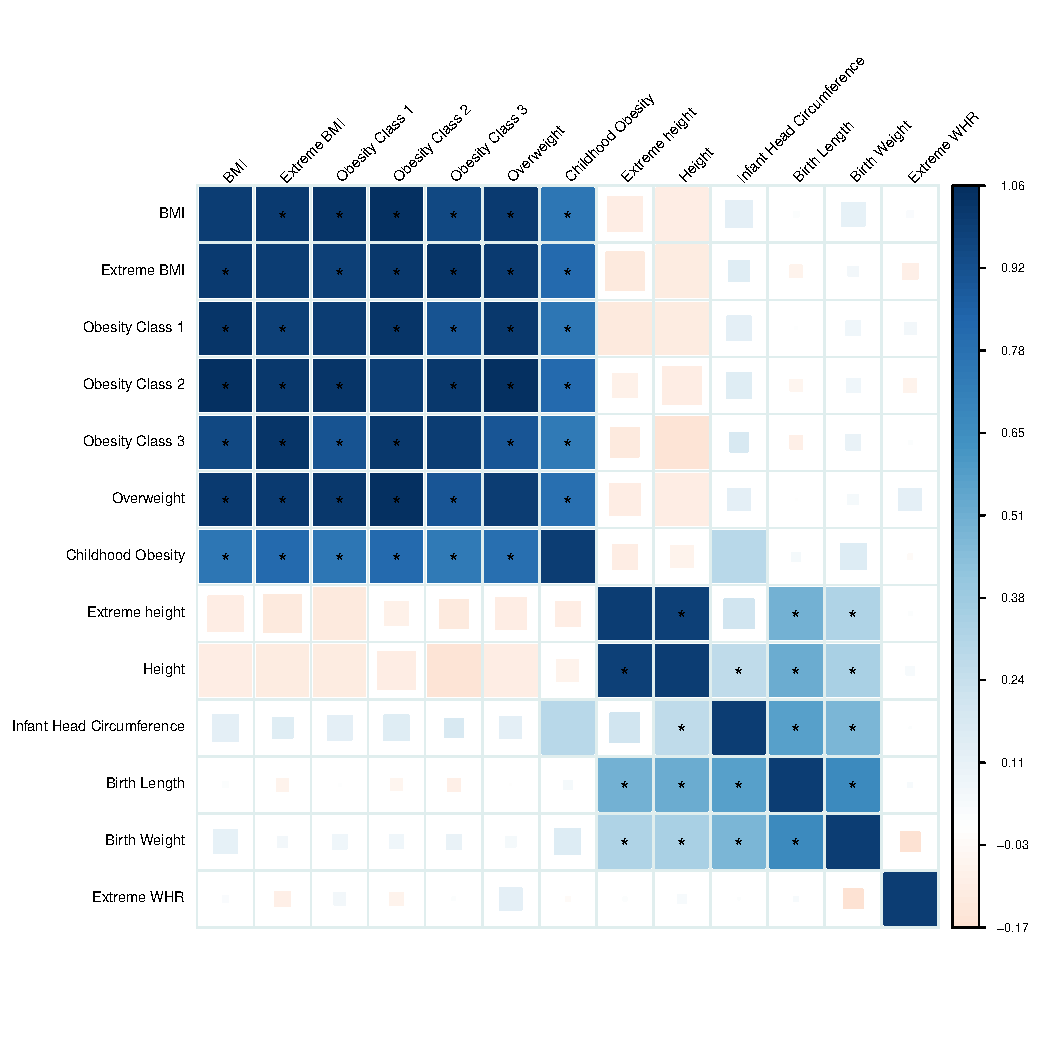
\includegraphics[scale=0.8]{figs/giant_supp.pdf}
\caption{\label{giant}\small{\textit{Genetic correlations among highly correlated anthropometric traits from studies by the GIANT and EGG consortia. The structure of the figure is the same as Figure \ref{Fig:300 Gencors} in the main text: 
blue corresponds to positive genetic correlations; red corresponds to negative genetic correlation. 
Larger squares correspond to more significant $p$-values.
Genetic correlations that are different from zero at 1\% FDR are displayed as full-sized squares. 
Genetic correlations that are significantly different from zero at significance level 0.05 after Bonferroni correction are given an asterisk.}}}
\end{centering}
\end{figure}
\newpage

\subsection*{Genetic Correlations among Smoking Traits}
\begin{figure}[!ht]
\begin{centering}
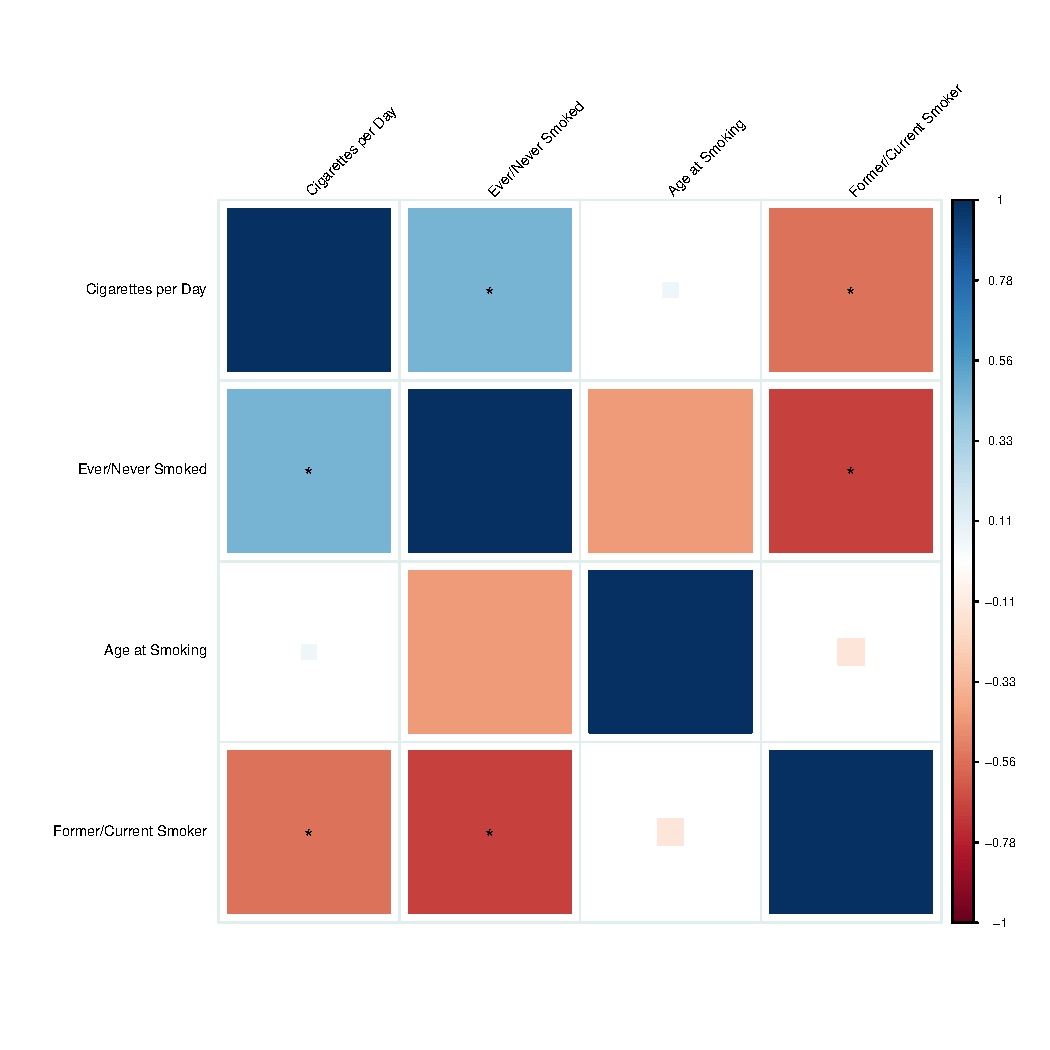
\includegraphics[scale=0.8]{figs/tag_supp.pdf}
\caption{\label{smoking}\small{\textit{Genetic correlations among highly correlated smoking-related traits from the Tobacco and Genetics (TAG) consortium. The structure of the figure is the same as Figure \ref{Fig:300 Gencors} in the main text: 
blue corresponds to positive genetic correlations; red corresponds to negative genetic correlation. 
Larger squares correspond to more significant $p$-values.
Genetic correlations that are different from zero at 1\% FDR are displayed as full-sized squares. 
Genetic correlations that are significantly different from zero at significance level 0.05 after Bonferroni correction are given an asterisk.}}}
\end{centering}
\end{figure}
\newpage

\subsection*{Genetic Correlations among Insulin-Related Traits}
\begin{figure}[!ht]
\begin{centering}
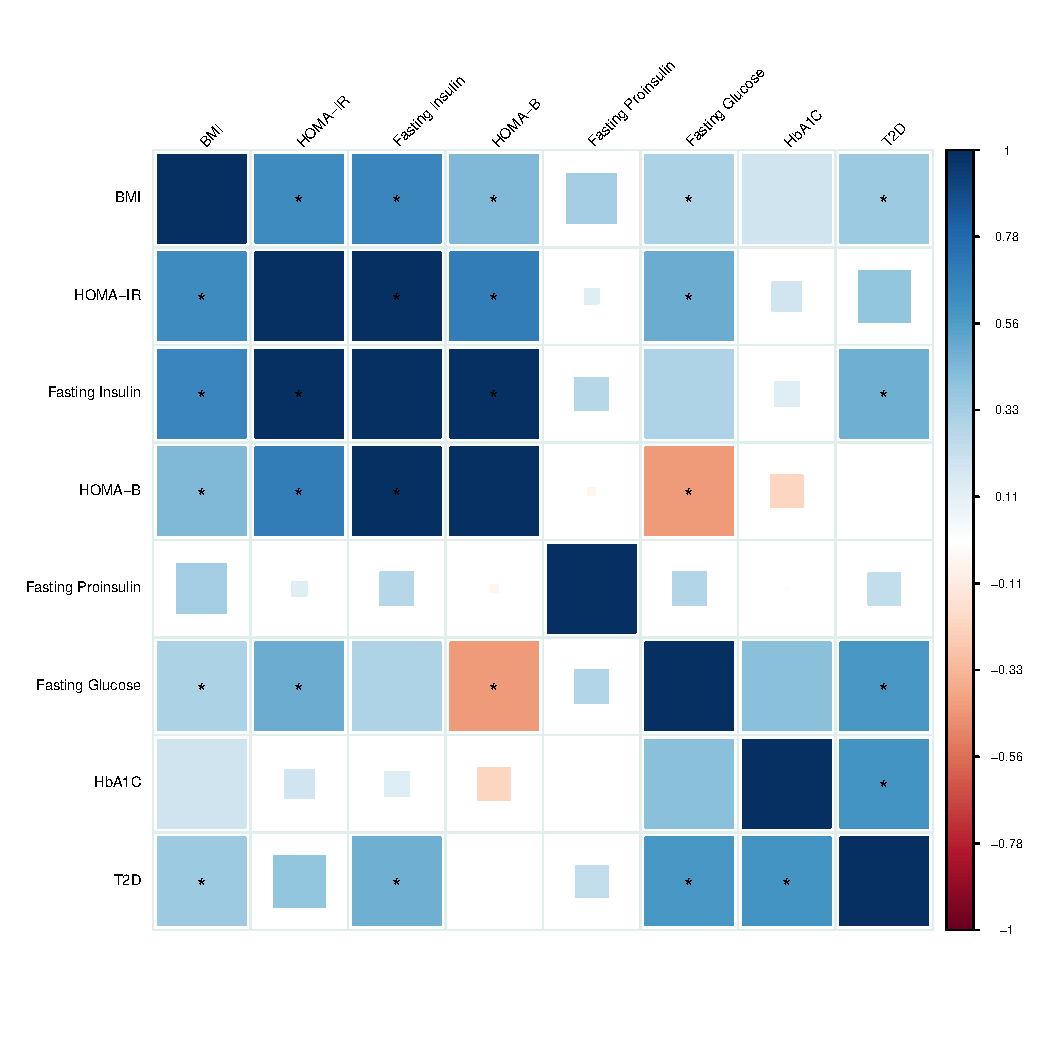
\includegraphics[scale=0.8]{figs/magic_supp.pdf}
\caption{\label{insulin}\small{\textit{Genetic correlations among highly correlated insulin-related traits from studies by the MAGIC consortium. The structure of the figure is the same as Figure \ref{Fig:300 Gencors} in the main text: 
blue corresponds to positive genetic correlations; red corresponds to negative genetic correlation. 
Larger squares correspond to more significant $p$-values.
Genetic correlations that are different from zero at 1\% FDR are displayed as full-sized squares. 
Genetic correlations that are significantly different from zero at significance level 0.05 after Bonferroni correction are given an asterisk.}}}
\end{centering}
\end{figure}
\newpage


\subsection*{Comparison of Metabolic Genetic Correlations from LDSC to Results from Vattikuti, et al}
\begin{figure}[!ht]
\begin{centering}
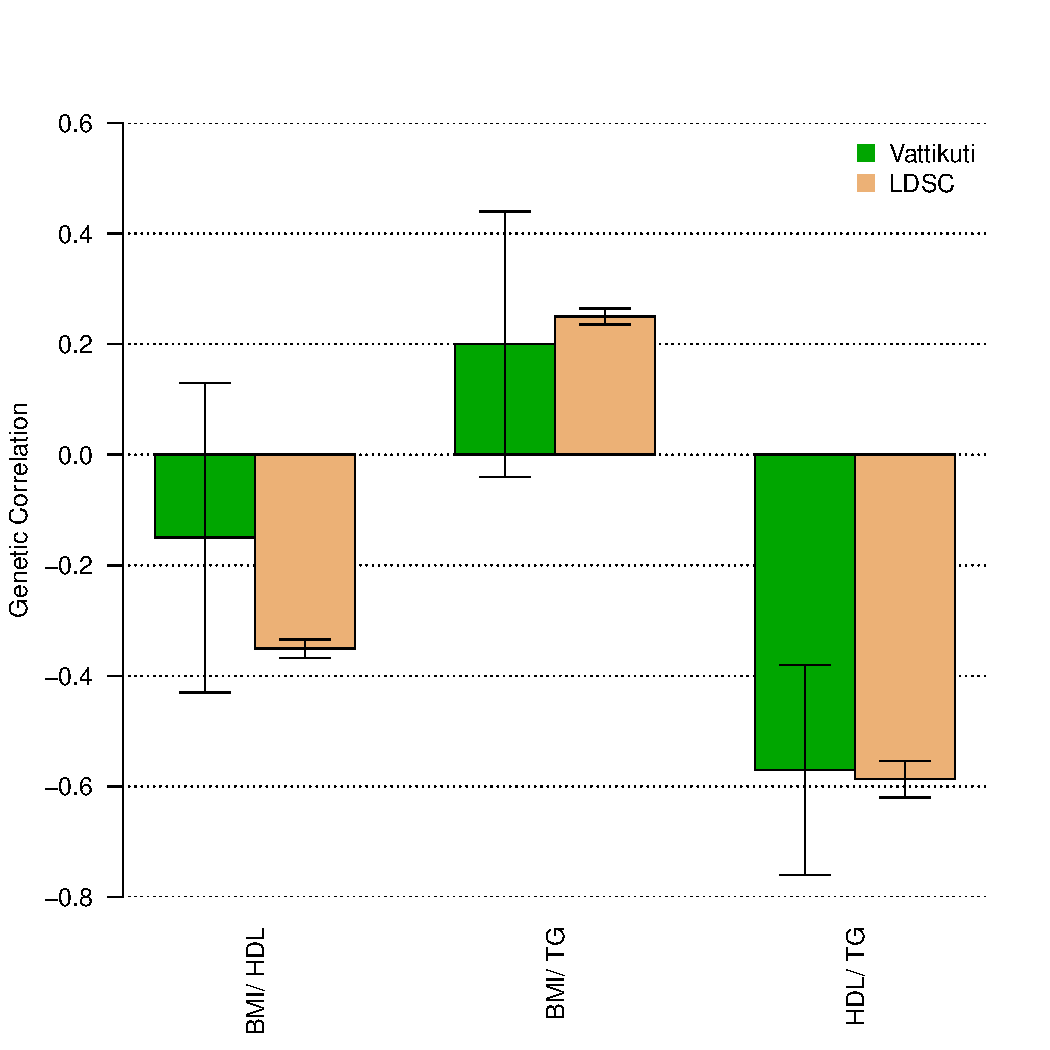
\includegraphics[scale=0.8]{figs/vattikuti.pdf}
\caption{\label{vattikuti}\small{\textit{This figure compares the estimates of genetic correlations between metabolic traits from table 3 of Vattikuti, et al. \cite{vattikuti2012heritability}
to the results obtained using LD Score regression (with much larger sample sizes) in this paper.}}}
\end{centering}
\end{figure}
\newpage

\subsection*{Schizophrenia / TG Conditional QQ Plot with and without the MHC}
\begin{figure}[!ht]
\begin{centering}
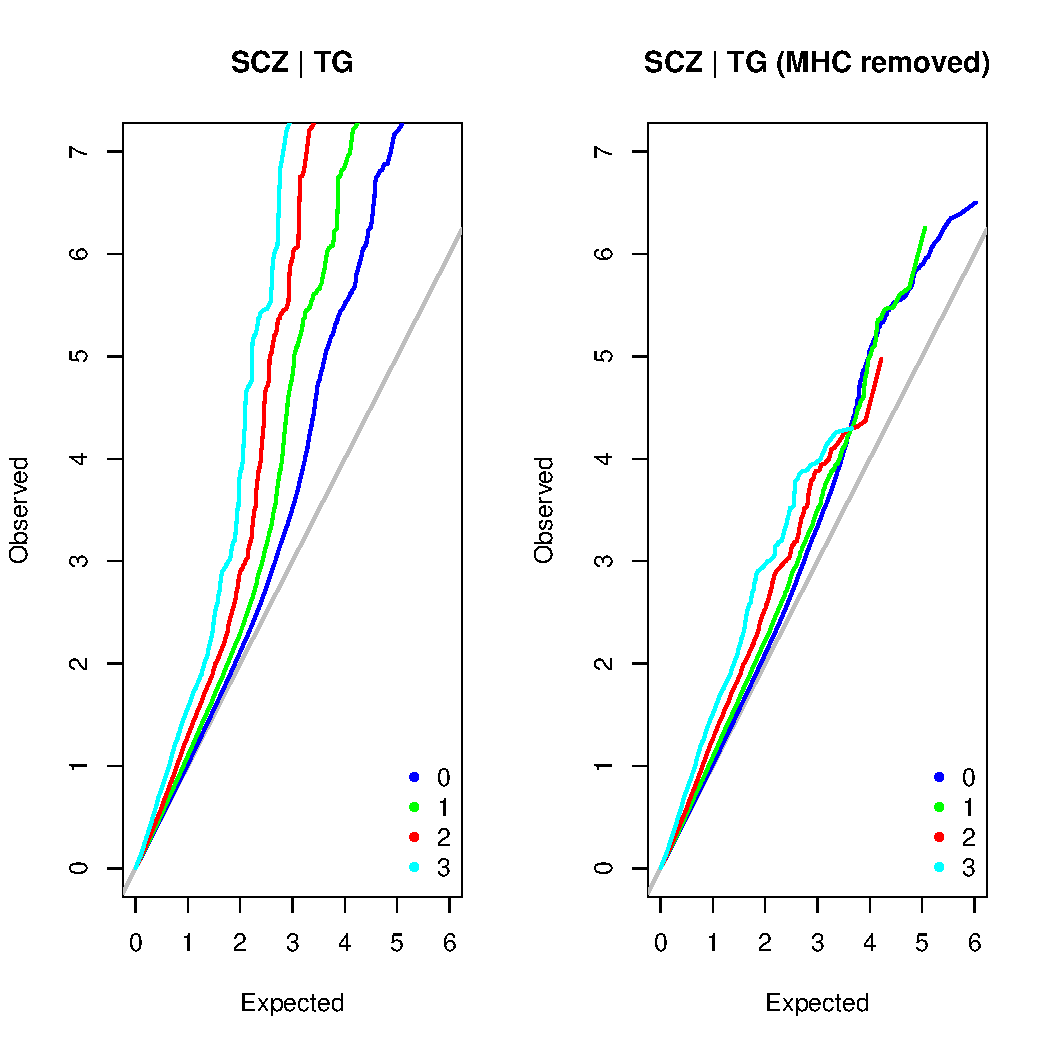
\includegraphics[scale=0.9]{figs/PGC1_pleiotropy_filter.png}
\caption{\label{qq_tg}\small{\textit{We reproduced the conditional QQ plot comparing schizophrenia (SCZ) and triglycerides (TG) from Andreassen et al. \cite{andreassen2013improved} (left). 
The major histocompatibility complex (MHC, approximately chr6, 25-35 MB) is
a genomic region featuring SNPs with exceptionally high LD Scores and the strongest GWAS association to schizophrenia.
Removing the MHC removes almost all signal from the conditional QQ plot (right), which is consistent with the 
near-zero genetic correlation between schizophrenia and TG estimated via LD Score regression.}}}
\end{centering}
\end{figure}
\newpage

%%%%%%%%%%%%%%%%%%%%%%%%%%%%%%%%%%%%%%%%%%%%%%%%%%%%%%%%%%%%%%%
\section*{Collaborators}
%%%%%%%%%%%%%%%%%%%%%%%%%%%%%%%%%%%%%%%%%%%%%%%%%%%%%%%%%%%%%%%

The members of the Schizophrenia Working Group of the Psychiatric Genetics Consortium are Stephan Ripke, Benjamin M. Neale, Aiden Corvin, James T.R. Walters, Kai-How Farh, Peter A. Holmans, Phil Lee, Brendan Bulik-Sullivan, David A. Collier, Hailiang Huang, Tune H. Pers, Ingrid Agartz, Esben Agerbo, Margot Albus, Madeline Alexander, Farooq Amin, Silviu A. Bacanu, Martin Begemann, Richard A. Belliveau, Jr., Judit Bene, Sarah E. Bergen, Elizabeth Bevilacqua, Tim B. Bigdeli, Donald W. Black, Anders D. B�rglum, Richard Bruggeman, Nancy G. Buccola, Randy L. Buckner, William Byerley, Wiepke Cahn, Guiqing Cai, Dominique Campion, Rita M. Cantor, Vaughan J. Carr, Noa Carrera, Stanley V. Catts, Kimberly D. Chambert, Raymond C.K. Chan, Ronald Y.L. Chen, Eric Y.H. Chen, Wei Cheng, Eric F.C. Cheung, Siow Ann Chong, C. Robert Cloninger, David Cohen, Nadine Cohen, Paul Cormican, Nick Craddock, James J. Crowley, David Curtis, Michael Davidson, Kenneth L. Davis, Franziska Degenhardt, Jurgen Del Favero, Lynn E. DeLisi, Ditte Demontis, Dimitris Dikeos, Timothy Dinan, Srdjan Djurovic, Gary Donohoe, Elodie Drapeau, Jubao Duan, Frank Dudbridge, Naser Durmishi, Peter Eichhammer, Johan Eriksson, Valentina Escott-Price, Laurent Essioux, Ayman H. Fanous, Martilias S. Farrell, Josef Frank, Lude Franke, Robert Freedman, Nelson B. Freimer, Marion Friedl, Joseph I. Friedman, Menachem Fromer, Giulio Genovese, Lyudmila Georgieva, Elliot S. Gershon, Ina Giegling, Paola Giusti-Rodrguez, Stephanie Godard, Jacqueline I. Goldstein, Vera Golimbet, Srihari Gopal, Jacob Gratten, Jakob Grove, Lieuwe de Haan, Christian Hammer, Marian L. Hamshere, Mark Hansen, Thomas Hansen, Vahram Haroutunian, Annette M. Hartmann, Frans A. Henskens, Stefan Herms, Joel N. Hirschhorn, Per Hoffmann, Andrea Hofman, Mads V. Hollegaard, David M. Hougaard, Masashi Ikeda, Inge Joa, Antonio Julia, Rene S. Kahn, Luba Kalaydjieva, Sena Karachanak-Yankova, Juha Karjalainen, David Kavanagh, Matthew C. Keller, Brian J. Kelly, James L. Kennedy, Andrey Khrunin, Yunjung Kim, Janis Klovins, James A. Knowles, Bettina Konte, Vaidutis Kucinskas, Zita Ausrele Kucinskiene, Hana Kuzelova-Ptackova, Anna K. Kahler, Claudine Laurent, Jimmy Lee Chee Keong, S. Hong Lee, Sophie E. Legge, Bernard Lerer, Miaoxin Li, Tao Li, Kung-Yee Liang, Jeffrey Lieberman, Svetlana Limborska, Carmel M. Loughland, Jan Lubinski, Jouko Lnnqvist, Milan Macek, Jr., Patrik K.E. Magnusson, Brion S. Maher, Wolfgang Maier, Jacques Mallet, Sara Marsal, Manuel Mattheisen, Morten Mattingsdal, Robert W. McCarley, Colm McDonald, Andrew M. McIntosh, Sandra Meier, Carin J. Meijer, Bela Melegh, Ingrid Melle, Raquelle I. Mesholam-Gately, Andres Metspalu, Patricia T. Michie, Lili Milani, Vihra Milanova, Younes Mokrab, Derek W. Morris, Ole Mors, Preben B. Mortensen, Kieran C. Murphy, Robin M. Murray, Inez Myin-Germeys, Bertram Mller-Myhsok, Mari Nelis, Igor Nenadic, Deborah A. Nertney, Gerald Nestadt, Kristin K. Nicodemus, Liene Nikitina-Zake, Laura Nisenbaum, Annelie Nordin, Eadbhard O'Callaghan, Colm O'Dushlaine, F. Anthony O'Neill, Sang-Yun Oh, Ann Olincy, Line Olsen, Jim Van Os, Psychosis Endophenotypes International Consortium, Christos Pantelis, George N. Papadimitriou, Sergi Papiol, Elena Parkhomenko, Michele T. Pato, Tiina Paunio, Milica Pejovic-Milovancevic, Diana O. Perkins, Olli Pietilinen, Jonathan Pimm, Andrew J. Pocklington, John Powell, Alkes Price, Ann E. Pulver, Shaun M. Purcell, Digby Quested, Henrik B. Rasmussen, Abraham Reichenberg, Mark A. Reimers, Alexander L. Richards, Joshua L. Roffman, Panos Roussos, Douglas M. Ruderfer, Veikko Salomaa, Alan R. Sanders, Ulrich Schall, Christian R. Schubert, Thomas G. Schulze, Sibylle G. Schwab, Edward M. Scolnick, Rodney J. Scott, Larry J. Seidman, Jianxin Shi, Engilbert Sigurdsson, Teimuraz Silagadze, Jeremy M. Silverman, Kang Sim, Petr Slominsky, Jordan W. Smoller, Hon-Cheong So, Chris C.A. Spencer, Eli A. Stahl, Hreinn Stefansson, Stacy Steinberg, Elisabeth Stogmann, Richard E. Straub, Eric Strengman, Jana Strohmaier, T. Scott Stroup, Mythily Subramaniam, Jaana Suvisaari, Dragan M. Svrakic, Jin P. Szatkiewicz, Erik Sderman, Srinivas Thirumalai, Draga Toncheva, Paul A. Tooney, Sarah Tosato, Juha Veijola, John Waddington, Dermot Walsh, Dai Wang, Qiang Wang, Bradley T. Webb, Mark Weiser, Dieter B. Wildenauer, Nigel M. Williams, Stephanie Williams, Stephanie H. Witt, Aaron R. Wolen, Emily H.M. Wong, Brandon K. Wormley, Jing Qin Wu, Hualin Simon Xi, Clement C. Zai, Xuebin Zheng, Fritz Zimprich, Naomi R. Wray, Kari Stefansson, Peter M. Visscher, Wellcome Trust Case Control Consortium, Rolf Adolfsson, Ole A. Andreassen, Douglas H.R. Blackwood, Elvira Bramon, Joseph D. Buxbaum, Anders D. Brglum, Sven Cichon, Ariel Darvasi, Enrico Domenici, Hannelore Ehrenreich, Tonu Esko, Pablo V. Gejman, Michael Gill, Hugh Gurling, Christina M. Hultman, Nakao Iwata, Assen V. Jablensky, Erik G. Jonsson, Kenneth S. Kendler, George Kirov, Jo Knight, Todd Lencz, Douglas F. Levinson, Qingqin S. Li, Jianjun Liu, Anil K. Malhotra, Steven A. McCarroll, Andrew McQuillin, Jennifer L. Moran, Preben B. Mortensen, Bryan J. Mowry, Markus M. Nthen, Roel A. Ophoff, Michael J. Owen, Aarno Palotie, Carlos N. Pato, Tracey L. Petryshen, Danielle Posthuma, Marcella Rietschel, Brien P. Riley, Dan Rujescu, Pak C. Sham, Pamela Sklar, David St. Clair, Daniel R. Weinberger, Jens R. Wendland, Thomas Werge, Mark J. Daly, Patrick F. Sullivan, and Michael C. O'Donovan.

The members of the Genetic Consortium for Anorexia Nervosa (GCAN) are
V Boraska, C S Franklin, J A B Floyd, L M Thornton, L M Huckins, L Southam, N William Rayner, I Tachmazidou, K L Klump, J Treasure, C M Lewis, U Schmidt, F Tozzi, K Kiezebrink, J Hebebrand, P Gorwood, R A H Adan, M J H Kas, A Favaro, P Santonastaso, F Fern�ndez-Aranda, M Gratacos, F Rybakowski, M Dmitrzak-Weglarz, J Kaprio, A Keski-Rahkonen, A Raevuori, E F Van Furth, M C T Slof-Op t Landt, J I Hudson, T Reichborn-Kjennerud, G P S Knudsen, P Monteleone, A S Kaplan, A Karwautz, H Hakonarson, W H Berrettini, Y Guo, D Li, N J Schork, G Komaki, T Ando, H Inoko, T Esko, K Fischer, K M�nnik, A Metspalu, J H Baker, R D Cone, J Dackor, J E DeSocio, C E Hilliard, J K O'Toole, J Pantel, J P Szatkiewicz, C Taico, S Zerwas, S E Trace, O S P Davis, S Helder, K B�hren, R Burghardt, M de Zwaan, K Egberts, S Ehrlich, B Herpertz-Dahlmann, W Herzog, H Imgart, A Scherag, S Scherag, S Zipfel, C Boni, N Ramoz, A Versini, M K Brandys, U N Danner, C de Kove, J Hendriks, B P C Koeleman, R A Ophoff, E Strengman, A A van Elburg, A Bruson, M Clementi, D Degortes, M Forzan, E Tenconi, E Docampo, G Escaram�s, S Jim�nez-Murcia, J Lissowska, A Rajewski, N Szeszenia-Dabrowska, A Slopien, J Hauser, L Karhunen, I Meulenbelt, P E Slagboom, A Tortorella, M Maj, G Dedoussis, D Dikeos, F Gonidakis, K Tziouvas, A Tsitsika, H Papezova, L Slachtova, D Martaskova, J L Kennedy, R D Levitan, Z Yilmaz, J Huemer, D Koubek, E Merl, G Wagner, P Lichtenstein, G Breen, S Cohen-Woods, A Farmer, P McGuffin, S Cichon, I Giegling, S Herms, D Rujescu, S Schreiber, H-E Wichmann, C Dina, R Sladek, G Gambaro, N Soranzo, A Julia, S Marsal, R a Rabionet, V Gaborieau, D M Dick, A Palotie, S Ripatti, E Wid�n, O A Andreassen, T Espeseth, A Lundervold, I Reinvang, V M Steen, S Le Hellard, M Mattingsda, I Ntalla, V Bencko, L Foretova, V Janout, M Navratilova, S Gallinger, D Pinto, S W Scherer, H Aschauer, L Carlberg, A Schosser, L Alfredsson, B Ding, L Klareskog, L Padyukov, C Finan, G Kalsi, M Roberts, D W Logan, L Peltonen, G R S Ritchie, P Courtet, S Guillame, I Jaussent, J C Barrett, X Estivill, A Hinney, P F Sullivan, D A Collier, E Zeggini, and C M Bulik.

The members of the Wellcome Trust Case Control Consortium 3 (WTCCC3) are
C A Anderson, J C Barrett, J A B Floyd, C S Franklin, R McGinnis, N Soranzo, E Zeggini, J Sambrook, J Stephens, W H Ouwehand, W L McArdle, S M Ring, D P Strachan, G Alexander, C M Bulik, D A Collier, P J Conlon, A Dominiczak, A Duncanson, A Hill, C Langford, G Lord, A P Maxwell, L Morgan, L Peltonen, R N Sandford, N Sheerin, N Soranzo, F O Vannberg, J C Barrett, D N A Genotyping, H Blackburn, W-M Chen, S Edkins, M Gillman, E Gray, S E Hunt, C Langford, a Nengut-Gumuscu, S Potter, S S Rich, D Simpkin, and Pa Whittaker.

The members of the Reprogen consortium are John RB Perry, Felix Day, Cathy E Elks, Patrick Sulem, Deborah J Thompson, Teresa Ferreira, Chunyan He, Daniel I Chasman, T�nu Esko, Gudmar Thorleifsson, Eva Albrecht, Wei Q Ang, Tanguy Corre, Diana L Cousminer, Bjarke Feenstra, Nora Franceschini, Andrea Ganna, Andrew D Johnson, Sanela Kjellqvist, Kathryn L Lunetta, George McMahon, Ilja M Nolte, Lavinia Paternoster, Eleonora Porcu, Albert V Smith, Lisette Stolk, Alexander Teumer, Natalia T�ernikova, Emmi Tikkanen, Sheila Ulivi, Erin K Wagner, Najaf Amin, Laura J Bierut, Enda M Byrne, JoukeJan Hottenga, Daniel L Koller, Massimo Mangino, Tune H Pers, Laura M YergesArmstrong, Jing Hua Zhao, Irene L Andrulis, Hoda AntonCulver, Femke Atsma, Stefania Bandinelli, Matthias W Beckmann, Javier Benitez, Carl Blomqvist, Stig E Bojesen, Manjeet K Bolla, Bernardo Bonanni, Hiltrud Brauch, Hermann Brenner, Julie E Buring, Jenny ChangClaude, Stephen Chanock, Jinhui Chen, Georgia ChenevixTrench, J. Margriet Coll�e, Fergus J Couch, David Couper, Andrea D Coveillo, Angela Cox, Kamila Czene, Adamo Pio D'adamo, George Davey Smith, Immaculata De Vivo, Ellen W Demerath, Joe Dennis, Peter Devilee, Aida K Dieffenbach, Alison M Dunning, Gudny Eiriksdottir, Johan G Eriksson, Peter A Fasching, Luigi Ferrucci, Dieter FleschJanys, Henrik Flyger, Tatiana Foroud, Lude Franke, Melissa E Garcia, Montserrat Garc�aClosas, Frank Geller, Eco EJ de Geus, Graham G Giles, Daniel F Gudbjartsson, Vilmundur Gudnason, Pascal Gu�nel, Suiqun Guo, Per Hall, Ute Hamann, Robin Haring, Catharina A Hartman, Andrew C Heath, Albert Hofman, Maartje J Hooning, John L Hopper, Frank B Hu, David J Hunter, David Karasik, Douglas P Kiel, Julia A Knight, VeliMatti Kosma, Zoltan Kutalik, Sandra Lai, Diether Lambrechts, Annika Lindblom, Reedik M�gi, Patrik K Magnusson, Arto Mannermaa, Nicholas G Martin, Gisli Masson, Patrick F McArdle, Wendy L McArdle, Mads Melbye Kyriaki Michailidou, Evelin Mihailov, Lili Milani, Roger L Milne, Heli Nevanlinna, Patrick Neven, Ellen A Nohr, Albertine J Oldehinkel, Ben A Oostra, Aarno Palotie,, Munro Peacock, Nancy L Pedersen, Paolo Peterlongo, Julian Peto, Paul DP Pharoah, Dirkje S Postma, Anneli Pouta, Katri Pylk�s, Paolo Radice, Susan Ring, Fernando Rivadeneira, Antonietta Robino, Lynda M Rose, Anja Rudolph, Veikko Salomaa, Serena Sanna, David Schlessinger, Marjanka K Schmidt, Mellissa C Southey, Ulla Sovio Meir J Stampfer, Doris St�ckl Anna M Storniolo, Nicholas J Timpson Jonathan Tyrer, Jenny A Visser, Peter Vollenweider, Henry V�lzke, Gerard Waeber, Melanie Waldenberger, Henri Wallaschofski, Qin Wang, Gonneke Willemsen, Robert Winqvist, Bruce HR Wolffenbuttel, Margaret J Wright, Australian Ovarian Cancer Study The GENICA Network, kConFab, The LifeLines Cohort Study, The InterAct Consortium, Early Growth Genetics (EGG) Consortium, Dorret I Boomsma, Michael J Econs, KayTee Khaw, Ruth JF Loos, Mark I McCarthy, Grant W Montgomery, John P Rice, Elizabeth A Streeten, Unnur Thorsteinsdottir, Cornelia M van Duijn, Behrooz Z Alizadeh, Sven Bergmann, Eric Boerwinkle, Heather A Boyd, Laura Crisponi, Paolo Gasparini, Christian Gieger, Tamara B Harris, Erik Ingelsson, MarjoRiitta J�rvelin, Peter Kraft, Debbie Lawlor, Andres Metspalu, Craig E Pennell, Paul M Ridker, Harold Snieder, Thorkild IA S�rensen, Tim D Spector, David P Strachan, Andr� G Uitterlinden, Nicholas J Wareham, Elisabeth Widen, Marek Zygmunt, Anna Murray, Douglas F Easton, Kari Stefansson, Joanne M Murabito, Ken K Ong.
\end{document}
